\chapter{Orchestrating Transformation Networks 
    \pgsize{40 p.}
}
\label{chap:orchestration}


\mnote{Transformation networks are composed of transformations and an application function}
A transformation network is composed of transformations and an application function, which executes the transformations in an order determined by an orchestration function.
In the previous chapters, we discussed how transformations can be defined and which properties they have to fulfill to be able to properly interoperate in a transformation network.
In the following, we will discuss how the other essential part, the application function can be realized.

\mnote{No notion of correctness for application functions}
Although the behavior of the application function is already defined in \autoref{def:applicationfunction}, we have shortly discussed that we cannot require correctness for this application function in the sense that it always yields consistent models for any given models and changes to them.
As we will see, this can either be because there is no execution order of the given transformations that yields consistent models or, even if it exists, it may not be possible to find it.

\mnote{We will discuss under which conditions transformation can be orchestrated to yield consistent models}
In this chapter, we will thus discuss under which conditions we can require the application function to return consistent models.
We derive an algorithm that realizes the application function and prove that it is not possible to ensure its termination without further restrictions to the transformations or the cases in which the algorithm is expected to return consistent models.
The discussion of different restriction options gives us the insight that none of them is applicable, because it restricts expressiveness of transformations and transformation networks too much.
Thus, we finally propose an algorithm that operates conservatively, i.e., if it returns models they are consistent but it may not always return consistent models although an execution of transformations that yields them exists.
That algorithm is supposed to improve the ability to find our why no execution order of transformations could be found although it existed.

\mnote{Proof for undecidability of the general orchestration problem, but practical algorithm for orchestration}
This chapter thus constitutes our contribution \contributionref{contrib:correctness:orchestration}, which consists of five subordinate contributions:
a discussion of the design of the application function with possible bounds for the number of executions and a notion of optimality, the derivation of an algorithm for the application function, for which we discuss termination and prove undecidability of the orchestration problem, a discussion of different strategies to restrict transformation that the orchestration problems becomes decidable, and finally first a discussion of options how to perform orchestration conservatively, as well as second the proposal of an algorithm that operates conservatively and help to find the reasons whenever no execution order of transformations yielding consistent models is found.
\todo{Finally update goals}
It answers the following research question:

\researchquestionrepeat{rq:correctness:orchestration}

\mnote{Contributions provide systemetic knnowledge on limitations of orchestration and a concrete algorithm}
While existing approaches to orchestrate transformations are restricted to specific topologies of transformation networks, our approach is supposed to not restrict the topology of transformations in any way.
Existing work proposes, for example, to define an execution order explicitly ~\cite{pilgrim2008a, vanhooff2007UniTI-MODELS} or to derive a topologic order~\cite{stevens2020BidirectionalTransformationLarge-SoSym}, which restricts the topologies to those in which a transformation needs to be executed only once.
We prove that is not possible to orchestrate arbitrary transformations such that they always yield consistent models when its possible.
We do, however, come up with an algorithm that is able to process transformation networks of arbitrary topology, which follows a specific orchestration strategy that does not necessarily find an execution order that yields consistent models whenever it exists, but instead is defined in way that it supports the transformation developer or user in finding the reason for the inability to find such an execution order.
On the one hand, this gives transformation developers systematic knowledge about limitations regarding the possibility to orchestrate transformations and, on the other hand, gives them a concrete algorithm for the orchestration to be readily applied.

% 1. Application function can return $\bot$ (or not terminate), what are the reasons that it needs to return $\bot$ or does not terminate?
% 1.1. In best case algorithm returns consistent models
% 1.2. If it does not, it may return $\bot$, return inconsistent models (is excluded by construction) or not terminate at all
% 1.3. When should it return $\bot$? Design Space for Functions
% 1.4. Why does it not terminate? Divergence/Alternation
% 2. Restriction to the Application Function
% 2.1. Execution Bound
% 2.2. Show Undecidability -> cannot find an orchestration although it exists
% 3. What restrictions can we make to transformation to, first, ensure that an orchestration exists and, second, it can be found?
% 3.1. Monotony


\section{Design Space for the Orchestration Function} % and orchestration function

\mnote{Undefined when application function is expected to return consistent models}
To recapitulate, the definition of an application function for transformation networks, given in \autoref{def:applicationfunction}, requires an application function $\appfunction{\orcfunction{\transformationset{T}}}$ to accept models and changes to them and yields either a set of models or $\bot$.
Whenever it returns a set of models, they must be achieved by applying the transformations in $\transformationset{T}$ of the network in an order determined by the orchestration function $\orcfunction{\transformationset{T}}$.
We then say that this execution order is an \emph{orchestration} of the transformations and that the execution of transformations in that order \emph{yields} those models.
The notion of correctness for the application function given in \autoref{def:applicationfunctioncorrectness} additionally requires the returned models to be consistent.
We did, however, not yet define when we expect the function to return consistent models and when we allow it to return $\bot$, as this requires further discussion of the alternatives, which we make in the following.

\mnote{Application function highly depends on orchestration function}
In fact, the application function highly depends on the results of the orchestration function.
If that function does not deliver an orchestration that yields consistent models, a correct application function may only return $\bot$.
Thus, we are specifically concerned with ensuring that the orchestration function finds an execution order that yields consistent models as often as possible.

\mnote{Orchestration function is allowed to return arbitrary long sequences of transformations}
The definition of an orchestration function allows it to determine an arbitrary long sequence of transformations, also including each transformation multiple times.
While we introduced this general notion to avoid unnecessary restrictions, in the following we show the necessity of having this general notion, rather than allowing each transformation to be executed only once, as proposed by existing work, such as \cite{stevens2020BidirectionalTransformationLarge-SoSym}.
From the insight that we need to allow transformations to be executed multiple times, we derive and discuss when we expect the application function to return consistent models, to finally come up with a notion of \emph{optimality} for the orchestration function determining the execution order.

% Discuss options for realizing the functions:
% Orchestration returns only sequence with each transformation executed once vs. arbitrary number of executions

% \begin{itemize}
%     \item We introduced a transformation network as a set of transformations, and an application function that uses an orchestration function to determine the execution order of the transformations for a given input
%     \item An application function may return $\bot$ or consistent models to be correct.
%     \item It may always return $\bot$ to be correct, this is however not what we want.
%     \item It would be intuitive to expect an application function to always return consistent models when there is an execution order of the transformations (i.e. an orchestration) that delivers consistent models.
%     \item So, we first investigate whether we can define a bound for the number of necessary transformation executions.
%     \item We there conclude, that we cannot restrict the number of necessary transformation execution
% \end{itemize}


\subsection{Execution Bounds}

\mnote{Ranges for possible numbers of transformation executions}
The possible number of executions for transformations of network range from a selected execution, e.g., in terms of spanning tree, over the execution of each transformation for one or a fixed number of times, to an arbitrary number of executions per transformations.
In the following, we will motivate why the single execution of each transformation is not sufficient in practice and prove that there can be cases in which it is not sufficient.

\mnote{Spanning trees are not sufficient}
The even stronger restriction to spanning trees is obviously not sufficient.
Consider the following consistency relations. For reasons of simplicity, we use \modellevelconsistencyrelations instead of fine-grained relations:
\begin{align*}
    & 
    \consistencyrelation{CR}{12} = \setted{\tupled{\model{m}{1}, \model{m}{2}}, \tupled{\model{m}{1}, \model{m}{2}'}, \tupled{\model{m}{1}', \model{m}{2}'}, \tupled{\model{m}{1}', \model{m}{2}''}} \\
    & 
    \consistencyrelation{CR}{13} = \setted{\tupled{\model{m}{1}, \model{m}{3}}, \tupled{\model{m}{1}, \model{m}{3}''}, \tupled{\model{m}{1}', \model{m}{3}}, \tupled{\model{m}{1}', \model{m}{3}'}} \\
    & 
    \consistencyrelation{CR}{23} = \setted{\tupled{\model{m}{2}, \model{m}{3}}, \tupled{\model{m}{2}', \model{m}{3}'}, \tupled{\model{m}{2}', \model{m}{3}''}, \tupled{\model{m}{2}'', \model{m}{3}}} 
\end{align*}
%We consider the set of these relations with their transposed ones: $\consistencyrelationset{CR} = \setted{\consistencyrelation{CR}{12}, \consistencyrelation{CR}{12}^T, \consistencyrelation{CR}{13}, \consistencyrelation{CR}{13}^T, \consistencyrelation{CR}{23}, \consistencyrelation{CR}{23}^T}$.
That set of relations is compatible according to \autoref{def:compatibility}, because for model there is a containing set of models that is consistent.
For the initial tuple of models $\tupled{\model{m}{1}, \model{m}{2}, \model{m}{3}}$, we consider a change that changes $\model{m}{1}$ to $\model{m}{1}'$.
Then we can distinguish tree possibly spanning trees of transformations that try to restore consistency, which we denote with $\transformation{T}_{12}, \transformation{T}_{13}, \transformation{T}_{23}$ for the according consistency relations.
Each tree consists of two transformations.
\begin{properdescription}
    \item[$\transformation{T}_{12}$, $\transformation{T}_{13}$:] 
    $\transformation{T}_{12}$ may change $\model{m}{2}$ to $\model{m}{2}'$. $\transformation{T}_{13}$ does nothing, because $\model{m}{1}'$ and $\model{m}{3}$ are already consistent to $\consistencyrelation{CR}{13}$.
    $\model{m}{2}'$ and $\model{m}{3}$ are, however, not consistent to $\consistencyrelation{CR}{23}$.
    \item[$\transformation{T}_{12}$, $\transformation{T}_{23}$:] 
    Like before, $\transformation{T}_{12}$ may change $\model{m}{2}$ to $\model{m}{2}'$. 
    $\transformation{T}_{23}$ may then change $\model{m}{3}$ to $\model{m}{3}''$. 
    $\model{m}{1}'$ and $\model{m}{3}''$ are, however, not consistent to $\consistencyrelation{CR}{13}$.
    \item[$\transformation{T}_{13}$, $\transformation{T}_{23}$:]
    $\transformation{T}_{13}$ may do nothing, because $\model{m}{1}'$ and $\model{m}{3}$ are already consistent to $\consistencyrelation{CR}{13}$.
    $\transformation{T}_{23}$ does also nothing, because $\model{m}{2}$ and $\model{m}{3}$ are still consistent to $\consistencyrelation{CR}{23}$.
    $\model{m}{1}'$ and $\model{m}{2}$ are, however, not consistent to $\consistencyrelation{CR}{12}$.
\end{properdescription}

\mnote{Each transformation needs to be executed at least once}
Thus, we need to execute each transformation at least once, because each transformation is only responsible for restoring its consistency relations and thus we cannot expect the resulting models to be consistent if some transformation were not executed, although the involved models were changed by other transformations.
However, restricting the execution to each transformation once is not appropriate either.
To show that, we consider examples that we derived from those we have already presented in \owncite{gleitze2020orchestration}, which used a different scenario context.

\begin{figure}
    \centering
    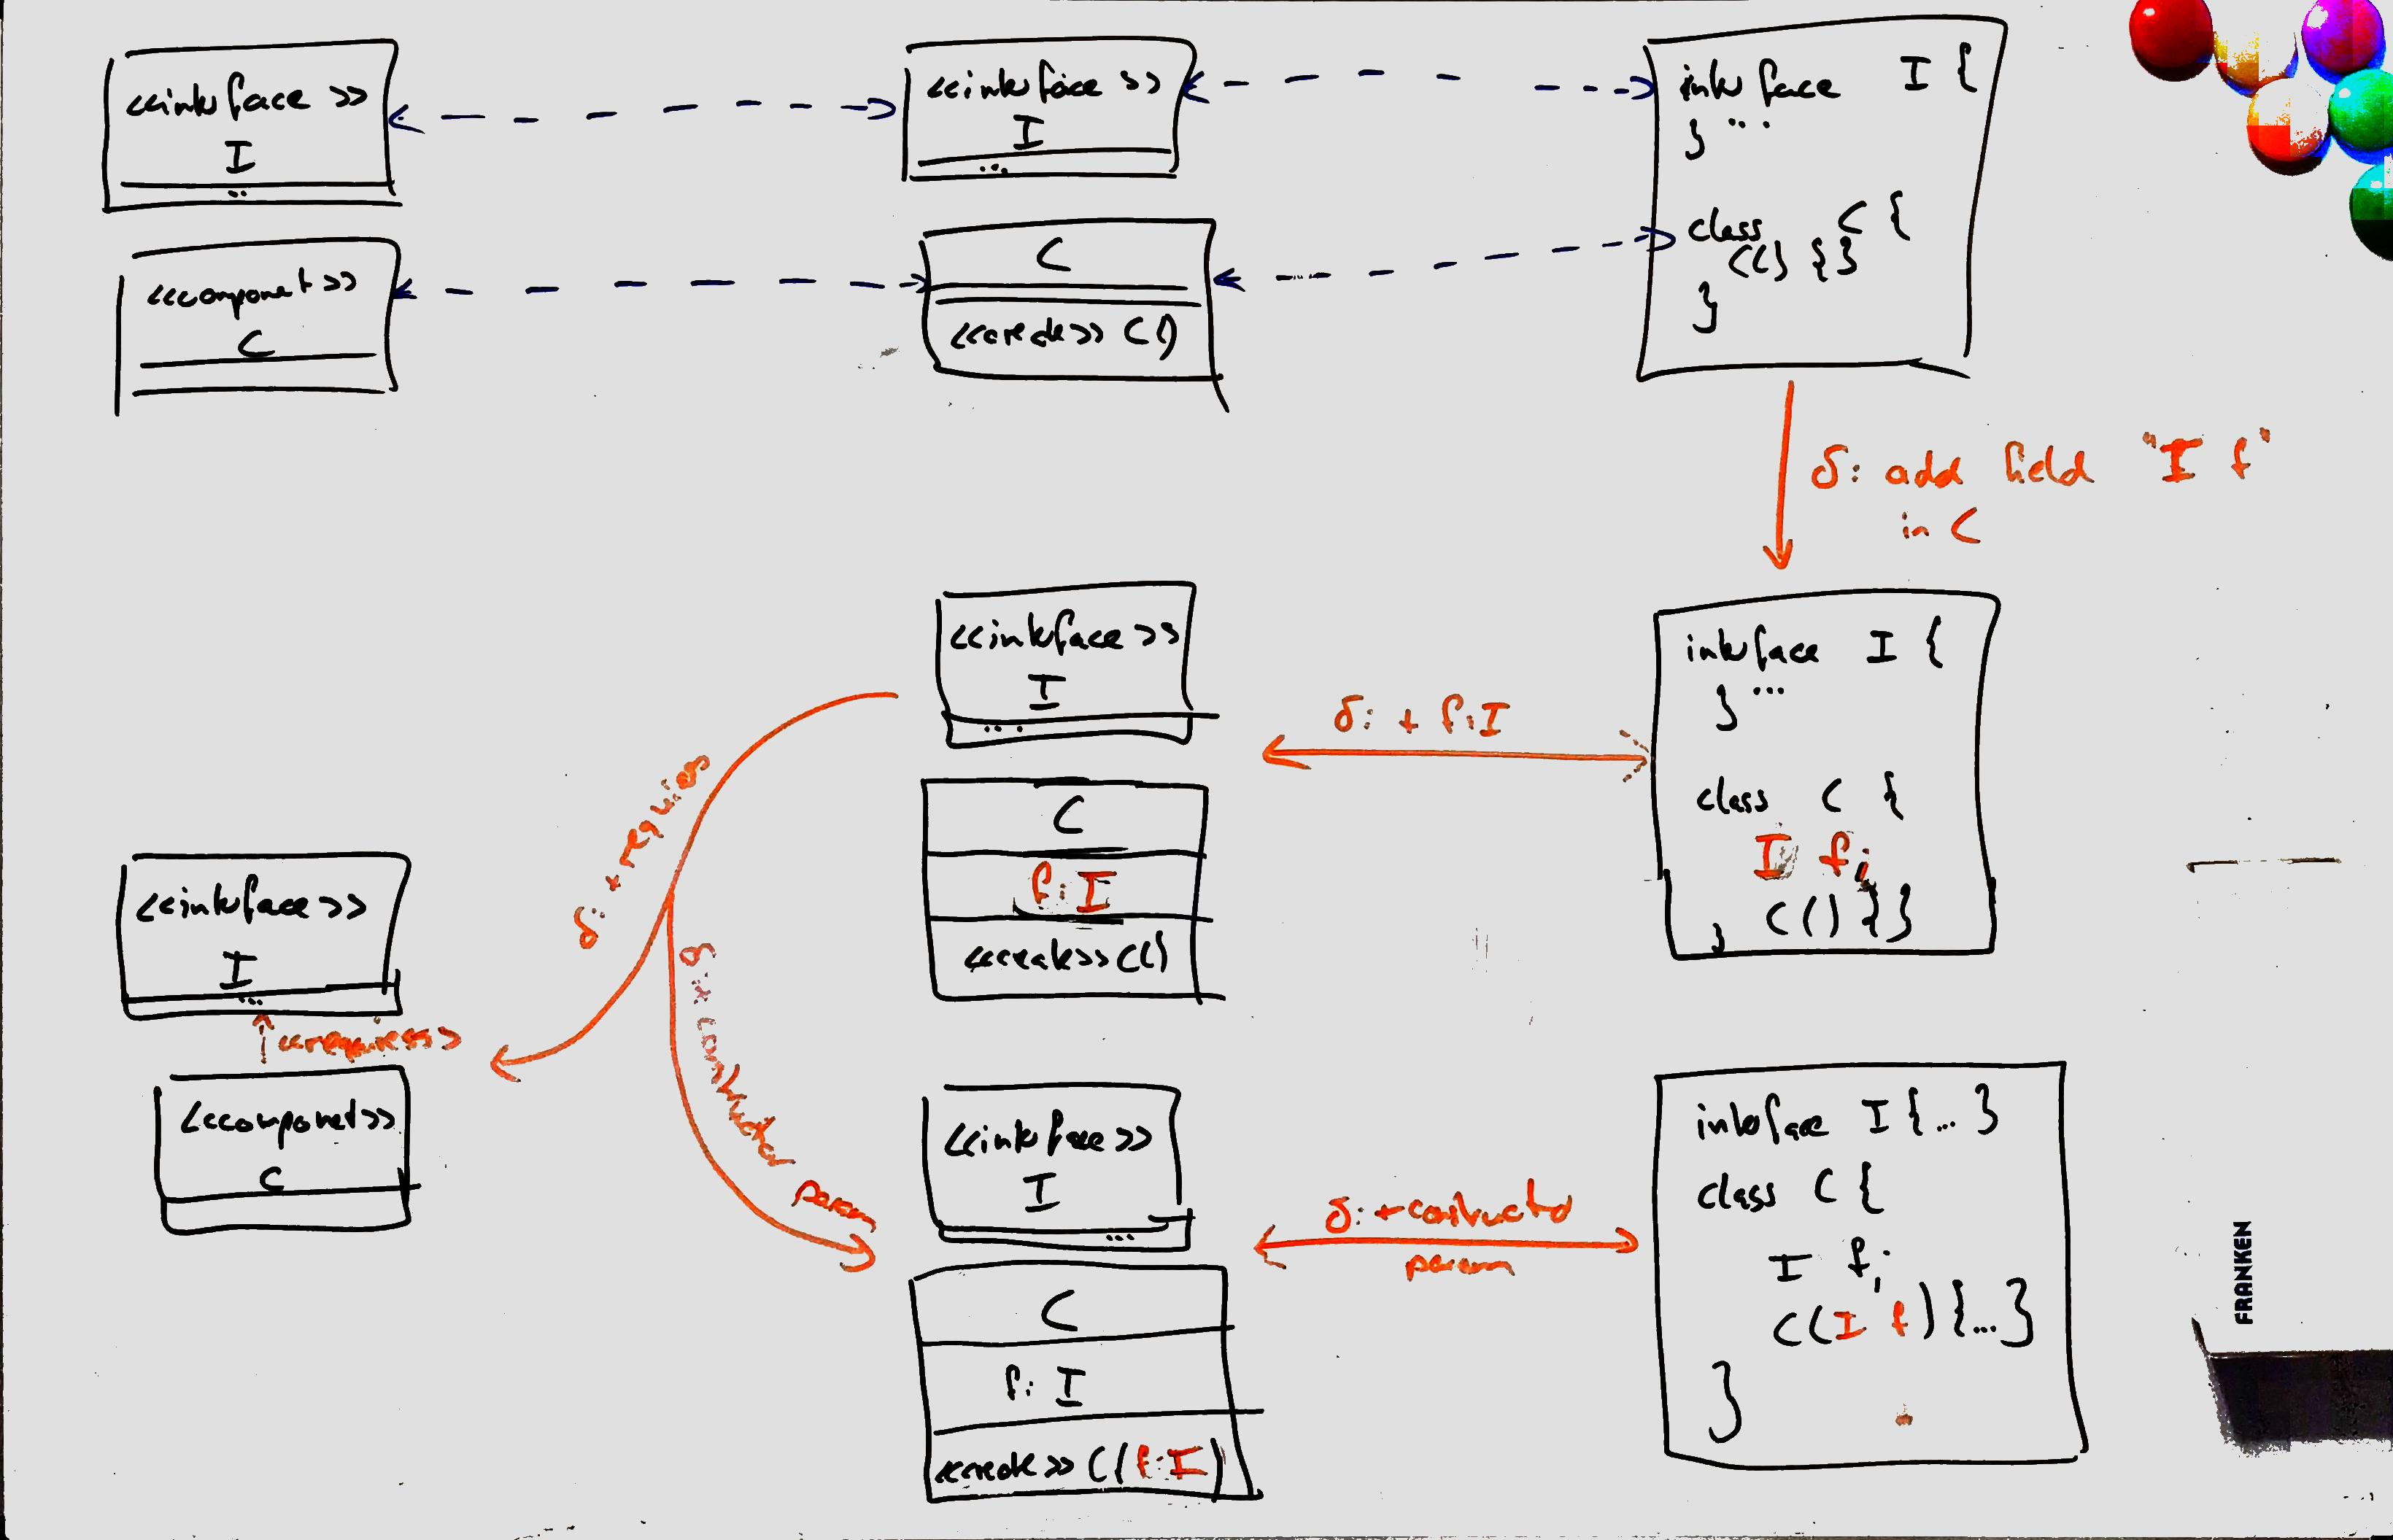
\includegraphics[width=\textwidth]{figures/correctness/orchestration/necessity_multiple_executions.jpg}
    \caption[Necessity of executing a transformation multiple times]{Necessity of executing a transformation multiple times.}
    \label{fig:orchestration:necessity_multiple_executions}
\end{figure}

\mnote{Example for component requires relation between \gls{PCM}, UML and Java}
Consider the example in \autoref{fig:orchestration:necessity_multiple_executions}, which describes the example depicted in \autoref{fig:introduction:scenario_duplicate_execution} within the introduction more precisely.
In the example, interfaces in UML and Java are related to architectural interfaces in a \gls{PCM} model.
\gls{PCM} components are realized by equally named classes in UML and Java.
Additionally, when a \gls{PCM} component requires an interface, this is realized by a field with the interface type in the component-realization class in UML and Java and an appropriate constructor argument.
Consistency is defined by transformations between \gls{PCM} and UML, as well as between UML and Java.

\mnote{Scenario requiring duplicate execution of one transformation}
In the scenario in \autoref{fig:orchestration:necessity_multiple_executions}, we begin with a consistent state of one interface and component, each realized by an interface and class, respectively, in both UML and Java.
A user then introduces a change of the Java code, in which he adds a field of the interface type to the component-realization class in Java.
The transformation between UML and Java propagates this change to the UML model, such that both models are consistent again.
The transformation between \gls{PCM} and UML then detects that the added field is of the type of an architectural interface, thus representing a requires relation between the corresponding component and the architectural interface. 
It adds the appropriate requires relation in the \gls{PCM} model, but also adds an appropriate parameter to the constructor of the component-realization class in UML, as required by the consistency relations.
This introduces a further inconsistency between the UML and the Java model, which requires the transformation between UML and Java to be executed again to also add that constructor parameter in the Java code.

\mnote{Cycles in transformation networks do not reduce necessary number of executions}
We simplified the example to the necessary core, although in practice a further transformation between \gls{PCM} and Java would be required, for example, to ensure that the field is set within the constructor.
One might argue that having a cycle of transformations between \gls{PCM}, UML and Java could resolve the problem, as the necessary second execution of the transformation between UML and Java is not necessary if the information is propagated from \gls{PCM} to Java.
This is, however, only true if exactly that order of transformations is chosen for execution and if the transformation between \gls{PCM} and Java does not introduce further information in the Java model that then needs to be propagated to UML.

\mnote{Synchronizing transformations can change models already processed by other transformation}
In general, it is always possible that transformations need to react to the changes performed by other, if they are not in some way aligned to each other.
This is due to the fact that a synchronizing transformation may change both models, thus if one transformation restores consistency between two models and another transformation reacts to that by restoring consistency between one of these models and another one, then both these models become changes, thus requiring the first transformation to process the newly created changes again.

\begin{figure}
    \centering
    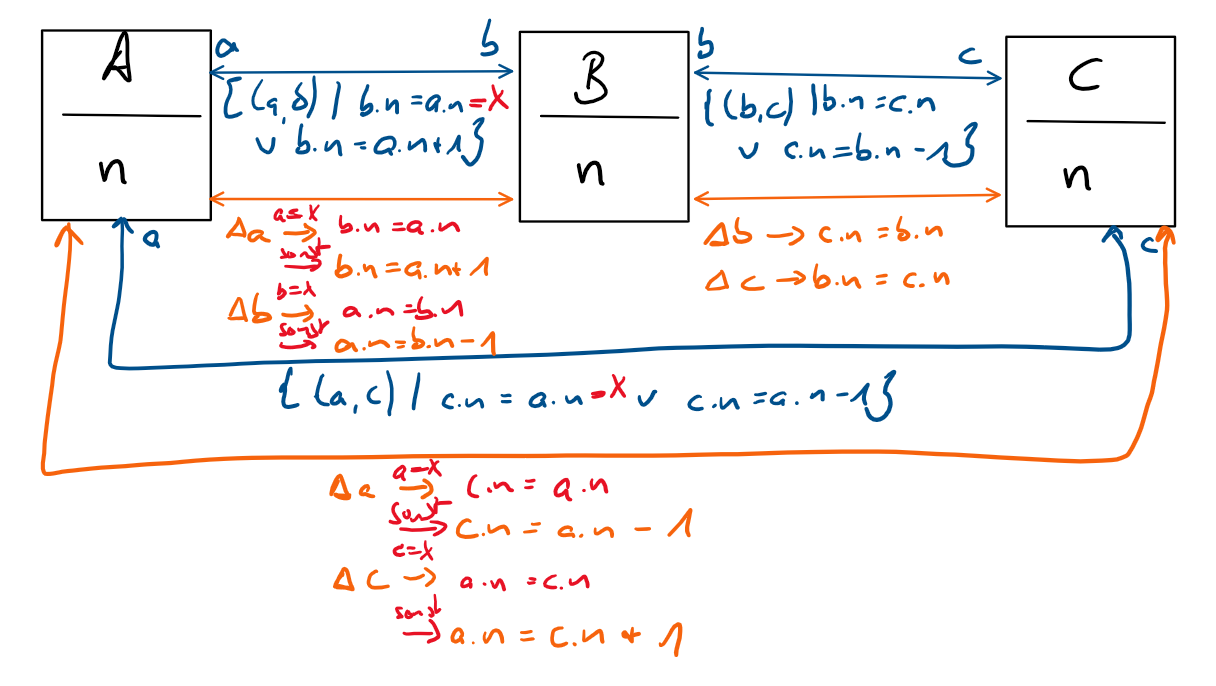
\includegraphics[width=\textwidth]{figures/correctness/orchestration/no_upper_bound_example.png}
    \caption[Example for arbitrary bounds of transformation execution]{Example for an arbitrary bound of necessary transformation execution.}
    \label{fig:orchestration:no_upper_bound}
\end{figure}

\mnote{Generalization to a theoretical incrementation example}
We can generalize the previous example to the one given in \autoref{fig:orchestration:no_upper_bound}.
It is an extension of the example given in \autoref{fig:synchronization:multiple_unidirectional_execution} for the necessity to execute the consistency preservation rules of a bidirectional transformation multiple times.
This also applies to the case in which multiple bidirectional transformations are combined.
The depicted relations and the informally defined consistency preservations rules require that elements \modelelement{A}, \modelelement{B} and \modelelement{C} with the same value of $n$ exist, and that for each \modelelement{A} with value $n$ a \modelelement{B} and \modelelement{C} with $n$ incremented by $1$ exist, except for the case that $n = x-1$.
In consequence, for an \modelelement{A} with $n = i$, all \modelelement{A}, \modelelement{B} and \modelelement{C} with $i \leq n < x$ need to exist.
This, obviously, requires the transformations to be executed $x-1-i$ times.

\mnote{Precise definition of transformation network}
We prove the informally given statement with the following precise definition of the transformations for a variable value of $x$.
Let $\class{A}{}, \class{B}{}, \class{C}{}$ be the classes depicted in \autoref{fig:orchestration:necessity_multiple_executions}.
\begin{align*}
    & 
    \metamodelinstanceset{M}{1} = \mathcal{P}(\metamodelinstances{\class{A}{}}), %\\
    %& 
    \metamodelinstanceset{M}{2} = \mathcal{P}(\metamodelinstances{\class{B}{}}), %\\
    %& 
    \metamodelinstanceset{M}{3} = \mathcal{P}(\metamodelinstances{\class{C}{}}) \\[1em]
    &
    \consistencyrelation{CR}{12} = \setted{\tupled{a,b} \in \metamodelinstances{\class{A}{}} \times \metamodelinstances{\class{B}{}} \mid b.n = a.n + 1 \neq x}, \consistencyrelationset{CR}_{12} = \setted{\consistencyrelation{CR}{12}, \consistencyrelation{CR}{12}^T} \\
    &
    \consistencypreservationrule{\consistencyrelationset{CR}_{12}}^{\rightarrow}(\model{m}{1}, \model{m}{2}, \change{\metamodel{M}{1}}) = \change{\metamodel{M}{2}} \\
    & \formulaskip
    \mathtext{with} \change{\metamodel{M}{2}}(\model{m}{2}) = \setted{b \in \metamodelinstances{\class{B}{}} \mid \exists a \in \change{\metamodel{M}{1}}(\model{m}{1}) : b.n = a.n + 1 \neq x} \\
    & 
    \consistencypreservationrule{\consistencyrelationset{CR}_{12}}^{\leftarrow}(\model{m}{2}, \model{m}{1}, \change{\metamodel{M}{2}}) = \change{\metamodel{M}{1}} \\
    & \formulaskip
    \mathtext{with} \change{\metamodel{M}{1}}(\model{m}{1}) = \setted{a \in \metamodelinstances{\class{A}{}} \mid \exists b \in \change{\metamodel{M}{2}}(\model{m}{2}) : b.n = a.n + 1 \neq x \land a \geq 0} \\
    &
    \transformation{T}_{12} = \tupled{\consistencyrelationset{CR}_{12}, \consistencypreservationrule{\consistencyrelationset{CR}_{12}}^{\rightarrow}, \consistencypreservationrule{\consistencyrelationset{CR}_{12}}^{\leftarrow}} \\[1em]
    & 
    \consistencyrelation{CR}{13} = \setted{\tupled{a,c} \in \metamodelinstances{\class{A}{}} \times \metamodelinstances{\class{C}{}} \mid c.n = a.n}, \consistencyrelationset{CR}_{13} = \setted{\consistencyrelation{CR}{13}, \consistencyrelation{CR}{13}^T} \\
    & 
    \consistencypreservationrule{\consistencyrelationset{CR}_{13}}^{\rightarrow}(\model{m}{1}, \model{m}{3}, \change{\metamodel{M}{1}}) = \change{\metamodel{M}{3}} \\
    & \formulaskip
    \mathtext{with} \change{\metamodel{M}{3}}(\model{m}{3}) = \setted{c \in \metamodelinstances{\class{C}{}} \mid \exists a \in \change{\metamodel{M}{1}}(\model{m}{1}) : c.n = a.n} \\
    & 
    \consistencypreservationrule{\consistencyrelationset{CR}_{13}}^{\leftarrow}(\model{m}{3}, \model{m}{1}, \change{\metamodel{M}{3}}) = \change{\metamodel{M}{1}} \\
    & \formulaskip
    \mathtext{with} \change{\metamodel{M}{1}}(\model{m}{1}) = \setted{a \in \metamodelinstances{\class{A}{}} \mid \exists c \in \change{\metamodel{M}{3}}(\model{m}{3}) : c.n = a.n} \\
    & 
    \transformation{T}_{13} = \tupled{\consistencyrelationset{CR}_{13}, \consistencypreservationrule{\consistencyrelationset{CR}_{13}}^{\rightarrow}, \consistencypreservationrule{\consistencyrelationset{CR}_{13}}^{\leftarrow}} \\[1em]
    &
    \consistencyrelation{CR}{23} = \setted{\tupled{b,c} \in \metamodelinstances{\class{B}{}} \times \metamodelinstances{\class{C}{}} \mid c.n = b.n}, \consistencyrelationset{CR}_{23} = \setted{\consistencyrelation{CR}{23}, \consistencyrelation{CR}{23}^T} \\
    & 
    \consistencypreservationrule{\consistencyrelationset{CR}_{23}}^{\rightarrow}, \consistencypreservationrule{\consistencyrelationset{CR}_{23}}^{\leftarrow} \mathtext{and} \transformation{T}_{23} \mathtext{accordingly} \\[1em]
    &
    \consistencyrelationset{CR} = \consistencyrelationset{CR}_{12} \cup \consistencyrelationset{CR}_{13} \cup \consistencyrelationset{CR}_{23} \\
    &
    \transformationset{T}_{inc} = \setted{\transformation{T}_{12}, \transformation{T}_{13}, \transformation{T}_{23}}
\end{align*}

\mnote{Proof that single execution of each transformation is not sufficient in scenario}
For these transformations, we are able to show that the transformation $\transformation{T}_{12}$ needs to be executed a minimal number of depending on $x$ for a specific input.
Thus, it is not sufficient to execute each transformation only once in this network.

\begin{lemma}[Minimal Number of Transformation Executions]
    \label{lemma:minimal_executions}
    Let $\transformationset{T}_{inc}$ be the previously defined set of transformations and let $\model{m}{1} = \model{m}{2} = \model{m}{3} = \emptyset$ be empty models and $\change{\metamodel{M}{1}} \in \changeuniverse{\metamodel{M}{1}}$ a change with $\change{\metamodel{M}{1}}(\model{m}{1}) = \setted{a \in \metamodelinstances{\class{A}{}} \mid a.n = 0}$.
    Then the result of every orchestration function $\orcfunction{\transformationset{T}_{inc}}$ with $\appfunction{\orcfunction{\transformationset{T}_{inc}}}(\tupled{\model{m}{1},\model{m}{2},\model{m}{3}},\tupled{\change{\metamodel{M}{1}},\identitychange,\identitychange}) \consistenttomath \consistencyrelationset{CR}$ contains $\transformation{T}_{12}$ at least $x-1$ times.
\end{lemma}
\begin{proof}
    $\appfunction{\orcfunction{\transformationset{T}_{inc}}}$ can only return consistent models when it applies the transformations in the order delivered by $\orcfunction{\transformationset{T}_{inc}}$ by definition in \autoref{def:applicationfunction}.
    We thus consider any order of transformations, as delivered by any orchestration function, to show that it contains $\transformation{T}_{12}$ at least $x-1$ times to deliver consistent models.
    
    Let $max_n(\model{m}{1},\model{m}{2},\model{m}{3}) = max\setted{e.n \mid e \in \model{m}{1} \cup \model{m}{2} \cup \model{m}{3}}$ be the maximal value of $n$ in any instance of \modelelement{A}, \modelelement{B} and \modelelement{C} in any given models $\model{m}{1}$, $\model{m}{2}$ and $\model{m}{3}$. In the following, we shortly note $max_n$ if the concrete models are currently not relevant.

    \begin{properdescription}
        \item[Executing $\transformation{T}_{13}$ and $\transformation{T}_{23}$ an arbitrary number of times does not increase $max_n$:]
        The transformations do only ensure that for any given models the returned models contain all elements with the same values of $n$ and do not introduce new elements with values of $n$ larger than the existing ones.
        \item[A single execution of $\transformation{T}_{12}$ increases $max_n$ by at most one:]
        There is no \modelelement{A} or \modelelement{B} with $n > max_n$.
        For every \modelelement{A} with $n < max_n$, $\transformation{T}_{12}$ creates, if necessary, a \modelelement{B} with value $n + 1 \leq max_n$, thus not increasing $max_n$.
        For every \modelelement{B} with $n \leq max_n$, it creates, if necessary, an \modelelement{A} with value $n-1 < max_n$.
        For every \modelelement{A} with $n = max_n$, a \modelelement{B} with value $n+1 = max_n + 1$ is creates, as long as $n \neq x-1$.
        For the newly created \modelelement{B}, no further elements needs to be created to fulfill the consistency relations.
        Thus, $max_n$ is, at most, increased by $1$.
        \item[ When $max_n(\model{m}{1},\model{m}{2},\model{m}{3}) < x-1$, then $\model{m}{1},\model{m}{2},\model{m}{3}$ are not consistent to $\consistencyrelationset{CR}$:]
        There is at least one element within the models with $n = max_n$.
        If the element with $n = max_n$ is an \modelelement{A}, then there must be a \modelelement{B} with value $n+1$, because of $\consistencyrelationset{CR}_{12}$ and because $n < x-1$.
        But since $n = max_n$, such a \modelelement{B} cannot exist, because otherwise $max_n = n+1$, so this is a contradiction.    
        If the element with $n = max_n$ is a \modelelement{C}, then $\consistencyrelationset{CR}_{13}$ requires an \modelelement{A} with the same value of $n$ to exist and the same argument as before leads to a contradiction.
        Finally, if the element with $n = max_n$ is a \modelelement{B}, then because of $\consistencyrelationset{CR}_{23}$ a \modelelement{C} with the same value must exist and then the same argument as before leads to a contradiction.
    \end{properdescription}

    In summary, we have shown that models $\model{m}{1},\model{m}{2},\model{m}{3}$ are only consistent to $\consistencyrelationset{CR}$ when $max_n(\model{m}{1},\model{m}{2},\model{m}{3}) \geq x-1$.
    Additionally, only $\transformation{T}_{12}$ increases $max_n$ and with each execution it only increases it by at most $1$.
    In consequence, starting with $max_n = 0$, we need at least $x-1$ executions of $\transformation{T}_{12}$ in an arbitrary sequence of the transformations in $\transformationset{T}_{inc}$ to achieve consistent models.
\end{proof}

\mnote{Example transformations can force network to perform an arbitrary number of executions}
We have proven that arbitrary transformation networks can require an arbitrary high number of executions of each transformations.
By selecting an appropriate $x$ in the used example network, we can force the network to perform at least $x$ executions of one transformation to yield a consistent tuple of models.
With this insight, it directly follows that we cannot find an approach to define orchestration functions that delivers sequences containing each transformation only once, when we do not ensure that if an order of transformations that yields consistent models exists, the approach is supposed to deliver it.

\begin{theorem}[Orchestration with Single Execution]
    \label{theorem:orchestration_single}
    For any set of transformations $\transformationset{T}$, there can be models $\modeltuple{m}$ and changes $\changetuple{}$ to them for which each possible orchestration function $\orcfunction{\transformationset{T}}$ with whom $\appfunction{\orcfunction{\transformationset{T}}}(\modeltuple{m}, \changetuple{})$ is consistent, delivers a sequence as $\orcfunction{\transformationset{T}}(\modeltuple{m}, \changetuple{})$ that contains at least one transformation twice.
\end{theorem}
\begin{proof}
    We know from \autoref{lemma:minimal_executions} that $\transformationset{T}_{inc}$ requires at least $2$ executions of $\transformation{T}_{12}$ for the inputs defined in \autoref{lemma:minimal_executions} when selecting $x \geq 3$.
    This proves the theorem by example.
\end{proof}

\mnote{Example generalizes practical scenario, thus single execution not supposed to be sufficient}
We know from \autoref{theorem:orchestration_single} that if we execute each transformation only once, we may exclude cases for which multiple executions of transformations would have led to a consistent tuple of models.
The example we have given in \autoref{fig:orchestration:necessity_multiple_executions} is a simplification of a realistic transformation scenario, which we generalized to the previous network with transformations $\transformationset{T}_{inc}$.
Thus, we can conclude that the insight is potentially relevant for realistic scenarios.
We should not restrict orchestration to execute each transformation only once, as there can be realistic scenarios in which multiple executions are necessary to find consistent models.
In the following, we thus, for first, allow an arbitrary number of executions of each transformation.

% Essential problem: One transformation may restore consistency between A and B and another between A and C. If then a transformation restores consistency between B and C, the resulting B' and C' may not be consistent A anymore.

% \todo{Beispiel warum mehrfache Ausführung nötig, warum also manche Infos erst durch andere bx reinkommen, die bei einer bx isoliert nicht relevant sind.}

% Bestehende Arbeiten (\cite{stevens2020BidirectionalTransformationLarge-SoSym}) schlagen auch vor eine Baumstruktur zu berechnen (Spannbaum), in dem nur entlang der Baumkanten die Transformationen ausgeführt werden. Dies ist jedoch eine starke Einschränkung daran, was die Transformationen ausdrücken können. Betrachtet man beispielsweise PCM, UML und Java, und hat eine Änderung in PCM. Dann könnte der Spannbaum entweder PCM -> UML -> Java sein, oder PCM -> UML + PCM -> Java. In ersterem Fall würde Verhaltensbeschreibung, die von PCM nach Java übertragen, aber in UML nicht dargestellt wird, nicht übertragen. Im zweiten Fall würde zusätzliche Information zwischen UML und Java nicht propagiert (Beispiel?) --> Hier sollte auf das Properties-Kapitel verwiesen werden, wo diese "Bottlenecks" erklärt sein sollten, inklusive einem Beispiel, die allgemein Baumstrukturen für Transformationsnetwerke ausschließen.

% Consequence: We cannot easily restrict the number of allowed executions. We can define networks that require an arbitrary number of executions.
% Also refer to the synchronization example, where we discussed that.
% Let us, for first, assume that transformations need an arbitrary number of executions.


\subsection{Expected Behavior} % Failure Cases} %When to Return $\bot$?}

\mnote{Necessity to define when application function returns $\bot$}
The application function is defined to return models only when they can be derived by applying transformations in an order delivered by the orchestration function and otherwise to return $\bot$.
In addition, we expect a \emph{correct} application function only to yield models that are consistent.
We did, however, not yet define under which conditions we expect the function not to return $\bot$, because there are different reasons why the function may not be able to deliver consistent models although we could expect it to do so.
In fact, with the current definition, the function is even considered correct if it always returns $\bot$, which is not practical.
Thus, we need to define when exactly we expect the function to return $\bot$.

\mnote{Reasons for not finding an orchestration that yields consistent models}
It might be intuitive to expect an application function to always return consistent models when the input models are consistent and when there is an execution order of the transformations, i.e., an orchestration, that delivers consistent models.
This, in consequence, would lead to the requirement that the orchestration function delivers a sequence of transformations whose application delivers consistent models whenever such a sequence exists for the given models and changes to them.
There can be different reasons why the orchestration function may not deliver such a sequence:
%When is it allowed or needed to return $\bot$?
%It may always return $\bot$ to be correct, this is however not what we want.
%We can distinguish three levels of reasons why the function may not be able to find consistent models:
\begin{properdescription}
    \item[Relations are incompatible:] If the consistency relations are incompatible, a user change may introduce an element for which no consistent models exist. In consequence, the transformation cannot be executed in an order such that the resulting models are consistent and still reflect the given user change.
    %(example with employee for which no consistent other models can be found)
    \item[No orchestration exists:] Even if the relations are compatible, transformations may be defined in a way that they make contradictory decisions for locally consistent solutions. Thus, for a given a change the consistency relations allow different ways to store consistency, of which the transformations always select a way that is not consistent to one of the other relations.
    Then no order of the transformations can restore consistency, although models exist that fulfill consistency for the given change.
    % (example with three options for name mapping with one overlapping, where each transformation always selects the one that is not appropriate for the other). We can further distinguish here whether there is always a change that cannot be processed by a CPR (then the change conflicts with the consistency relations and thus has to be rejected like any change may need to be rejected), or whether an arbitrary long sequence of transformations exists that can be applied but does never yield a consistent set of models.
    \item[No orchestration found:] Finally, although an order of transformations for given changes exists that delivers consistent models, the orchestration function may not deliver it. 
    %finally, the application/orchestration may not be able to find an order of transformations that leads to a consistent state although it exists.
\end{properdescription}

\mnote{Reasons induce each other}
These reasons can be considered at different levels, because each of them induces the next, i.e., if there is no orchestration, it cannot be found, and having contradictory relations, there exists no orchestration for some of the changes.
In the end, all of them lead to the situation that no orchestration can be found and, thus, the orchestration function is not able to deliver it.

\mnote{Compatibility can be assumed, existence of an orchestration cannot}
The initially given intuitive requirement that the orchestration function delivers a transformation sequence that yields consistent models whenever it exists would thus assume that the first two levels do not occur and then require the orchestration function to ensure the third.
While we can assume compatibility of the relations, as we discussed how to analyze it in \autoref{chap:compatibility}, we cannot assume that an orchestration does always exists, as we will see in the following.

\mnote{Compatibility does not ensure existence of orchestration}
Although compatibility reduces the chance that an orchestration function does not deliver a transformation sequence that yields consistent models, as we have motivated with the scenario depicted in \autoref{fig:compatibility:unwanted_behavior}, it does not ensure that there is always such a sequence of transformations that the orchestration function can find.
In general, this is always the case when consistency relations define different options for consistency, i.e., they allow the existence of different corresponding elements to consider the models consistent.
Compatibility ensures that there is an overlap of these corresponding elements, such that for every element, for which consistency is restricted, consistent models can be found.
If, however, the consistency preservation rules of the transformations always restore consistency by introducing corresponding elements that are not in this overlap, each transformation will restore consistency locally to its consistency relation, but they can, together, never restore consistency to all consistency relations.

\mnote{Consistency preservation rules need to select overlapping options in consistency relations}
Consider the situation that we have three metamodels $\metamodel{A}{}$, $\metamodel{B}{}$ and $\metamodel{C}{}$ with instances $\model{a}{i}$, $\model{b}{i}$ and $\model{c}{i}$.
Let us assume that those models are uniquely indexed by $i$ and we defined the following consistency relations:
\begin{align*}
    &
    \consistencyrelation{CR}{AB} = \setted{\tupled{\model{a}{i}, \model{b}{k}} \mid k = i} \\
    &
    \consistencyrelation{CR}{AC} = \setted{\tupled{\model{a}{i}, \model{c}{l}} \mid l = i \lor l = i+1} \\
    &
    \consistencyrelation{CR}{BC} = \setted{\tupled{\model{b}{k}, \model{c}{l}} \mid l = k+1 \lor l = k+2}
\end{align*}
This induces the set of consistent models $\setted{\tupled{\model{a}{i}, \model{b}{k}, \model{c}{l}} \mid  i = k = l-1}$, which is given to all three consistency relations.
Thus for any given model we are able to find instances of the other metamodels that are consistent to all consistency relations.
If we define consistency preservation rules for these consistency relations, the ones for $\consistencyrelation{CR}{AC}$ and $\consistencyrelation{CR}{BC}$ may decide between two models to restore consistency.
If $\consistencyrelation{CR}{AC}$ does always select $\model{c}{i}$ for $\model{a}{i}$ and vice versa, and if $\consistencyrelation{CR}{BC}$ does always select $\model{c}{i+2}$ for $\model{a}{i}$ and vice versa, no orchestration of the transformations will yield consistent models, because they never select those models that are in the overlap of the consistency relations.

\begin{figure}
    \centering
    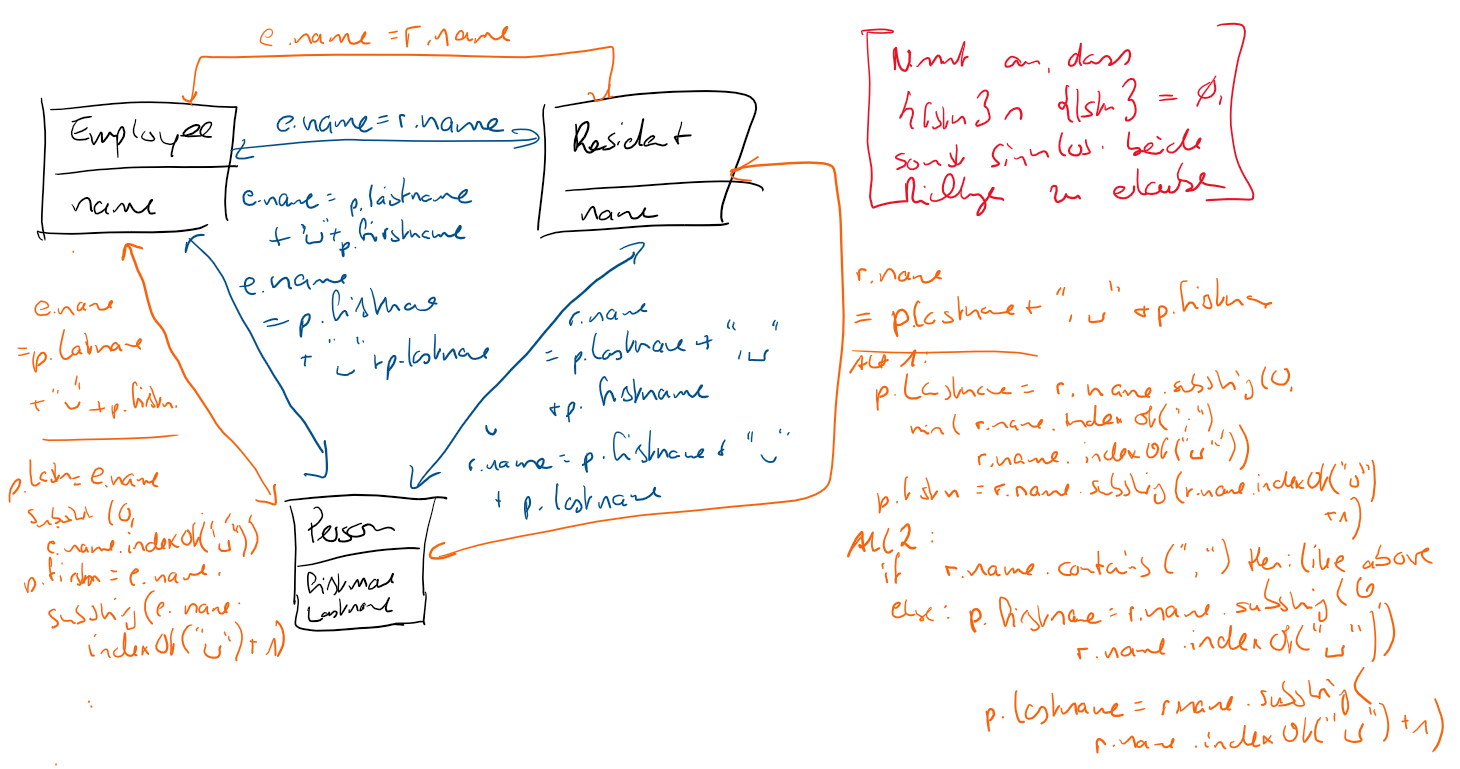
\includegraphics[width=\textwidth]{figures/correctness/orchestration/no_orchestration.png}
    \caption[Consistency preservation rules without orchestration]{Consistency relations with options for corresponding elements leading to consistency preservation rules of which no orchestration yields consistent models.}
    \label{fig:orchestration:no_orchestration}
\end{figure}

\mnote{Running example with consistency relations for name composition}
We have already given an abstract example for that problem in \autoref{fig:correctness:no_execution_order}. \autoref{fig:orchestration:no_orchestration}, in addition, demonstrates this situation at a derivation of the running example.
The consistency relation between employees and residents ensures that for each resident and employee there is corresponding other element with the same name.
The consistency relations between employees and persons and between residents and persons ensure that for each person there is a corresponding employee and resident, respectively, but they allow different relations of their names.
While both consider elements corresponding if the name of an employee and resident, respectively, are the concatenation of the first and last name of a person, an employee is also allowed to have the inverse concatenation of last and first name, whereas a resident is also allowed to have this inverse concatenation, but with an additional separation of the last and first name with a comma.
These options for the consistency relations provide further degrees of freedom for each transformation on its own, as they allow, for example, employee names to be encoded differently.
This can, for example, be reasonable if the order of first and last name is not relevant in a model managing employees.
In combination with the other consistency relations, however, the only employees, residents and persons that are considered consistent to all of the consistency relations are those having the same names with the concatenation of first and last name.
Nevertheless, these consistency relations are compatible, because for each possible condition element, i.e., for every possible employee, person and resident, there are consistent models that contain them.

\mnote{Relations in the running example without orchestration that yields consistent models}
Consistency relations that preserve these consistency relations need to to choose one of the given options for the names of corresponding employees, residents and persons.
\autoref{fig:orchestration:no_orchestration} sketches consistency preservation rules that make such a selection.
The rules with alternative 1 ensure that for each employee, resident and persons corresponding elements exist, which fulfill those relations of the names that are conflicting.
This means, the employee name is the concatenation of the last and first name of a person, whereas the resident name contains an additional comma in that concatenation.
In the other direction, the names of employees and residents are split at the appropriate indices, given by the whitespace and comma, respectively, to calculate the required first and last name of a person.
In consequence, there is no execution sequence of the transformations that results in consistent models, because the execution of the transformation between employees and persons always leads to a violation of the consistency relation between residents and persons and vice versa.
This is because the transformation between person and resident always introduces a comma in the resident name, which is then appended to the last name by the transformation between employee and persons.
A repeated execution of the transformation repeatedly appends that comma.
On the other hand, the execution of any of the transformation does never lead to the introduction of a person that fulfills the non-conflicting conditions of both consistency relations by simply containing a first and last name, which is represented as concatenation of first and last name in both an employee and resident.
This is concrete example for the previously discussed abstract situation that of different options in consistency relations always the non-overlapping ones are chosen by the consistency preservation rules.

\mnote{Alternative relations in the running example}
If we consider the alternative 2 for the consistency preservation rule between persons and residents, we can always find an orchestration that yields consistent models.
The alternative rule decides how consistency is ensured based on the existence of a comma within the resident name.
If a comma is present, the name relation containing a comma is used, and otherwise the simple concatenation of first and last name is assumed.
For an employee, first execution the transformation from employees to residents and afterwards the one from residents to persons ensures that all consistency relations are fulfilled, because the one between residents and persons sets first and last name of a person according to the relations that is also fulfilled between person and employee, because the name does not contain a comma.
For a person, first executing the transformation from persons to employees and then following the process above also ensures consistency.
Finally, for a resident, we can, for example, first apply the transformation between residents and employees and then the one between residents and persons, resulting in consistent models due to the same reasons as above.

\mnote{Only specific orchestrations yield consistent models}
Although there are execution orders of the transformations that yield consistent models with the consistency preservation rule defined as alternative 2, not every execution order leads to consistent models.
In the scenarios discussed above, we have ensured that the transformation between residents and persons is executed for a resident first.
If that transformation is first executed for a person, then a comma is added, which leads to the subsequent application of the same consistency preservation rules as with alternative 1, meaning that no further execution order yields consistent models.

\mnote{Necessity to find orchestrations that yield consistent models}
No matter whether exactly those consistency relations and preservation rules for them may occur in an actual transformation network, they exemplify the general situation of having consistency preservation rules that select one of different options provided by the consistency relation to introduced corresponding elements to restore consistency.
The example shows that whether or not an order of transformations exists that yields consistent models in such a situation depends on whether at least one transformation selects an option that is consistent to other consistency relations as well.
It also shows that even if an execution order exists, not all execution orders yield consistent models, thus we need to be able to find one that does.

\mnote{Resolvability as the existence of an orchestration}
In accordance with existing work \cite{stevens2020BidirectionalTransformationLarge-SoSym}, we call a given set of models and changes \emph{resolvable} by a transformation network, if an orchestration exists.
In contrast to existing work, we do, however, not restrict ourselves to a single execution of each transformation, as we have motivated before.

\mnote{Necessity to deal with unresolvability}
We have to accept that transformation networks may be unresolvable, i.e., that there is no orchestration for the transformations that yields consistent models.
Ensuring that a network is resolvable for any changes would lead to restrictions for the individual transformations, which would especially require different transformations to be aligned with each other.
Since that conflicts our assumption of independent development and modular reuse, we do not focus on that problem, but accept that it can occur and instead focus on how we can find an orchestration if it exists. 

\mnote{Optimality property of orchestration function}
In conclusion, we expect the application function to deliver consistent models whenever an orchestration that yields them exists.
Thus, we want to ensure that the orchestration function is able to always find such an orchestration, if it exists.
We define this as an \emph{optimality} property in the following.

% "has a resolution" bei Stevens entspricht im Prinzip Kompatibilität
% "is resolvable" bei Stevens entspricht im Prinzip "orchestration exists"

% In accordance to existing work, such as \cite{stevens2020BidirectionalTransformationLarge-SoSym}, we call a given set of models and changes \emph{resolvable} by the transformation network, if there exists a sequence of the transformations such that the resulting models are consistent.
% We do, however, not restrict ourselves to a single execution of each transformation but allow them to be executed multiple times (as motivated before).
% Orchestration ermittelt eine "Resolution" (siehe bestehende Arbeiten~\cite{stevens2020BidirectionalTransformationLarge-SoSym}), also eine Ausführungsreihenfolge, zumindest wenn man sie als "korrekt" bezeichnet.

% Argumentation:
% Compatibility können wir fordern, dass eine Orchestrierungsstrategie existiert aber nicht. 

% We can avoid the first by requiring compatibility.
% We need to make restrictions to the transformation to resolve the second. We do, however, probably need to require them to know about the other transformations to avoid that. Finally, we will have to deal with that situation and then inform the user about the problem.
% We investigate whether we can always guarantee to find an orchestration if it exists.
% For now, we focus on the last problem, since that is a problem of the application and orchestration function, rather than the problem that no orchestration may exist at all.

% DECIDED THAT THE FOLLOWING IS NOT AN OPTINO BUT THE SECOND IS DEFINITE.
% Now we have these options:
% \begin{itemize}
%     \item We accept that there is no orchestration or that the strategy does not find it in specific situations, than we only need to consider that the strategy must always terminate.
%     We could, for example, change the algorithm such that it always returns $\bot$, which is correct, or terminates after executing each transformation once.
%     \item We define a precise criterion when the strategy is allowed to return $\bot$. Most intuitively, one might say that it should only return $\bot$ whenever no orchestration exists.
% \end{itemize}



\subsection{Optimal Orchestration}

% An application function that delivers consistent models whenever an orchestration exists that yields them is what we would assume \emph{optimal}.
% Recall that $\generalizationfunction{\metamodeltuple{M},\transformation{t}}$ is the generalization function that applies a transformation, which is only defined for two models, to a model tuple that instantiate all metamodels in $\metamodeltuple{M}$.

% \begin{definition}[Optimal Transformation Application Function]
%     Let $\transformationset{T}$ be a set of transformations for a set of metamodels $\metamodeltuple{M} = \tupled{\metamodelsequence{M}{n}}$.
%     We say that an application function $\appfunction{\orcfunction{\transformationset{T}}}$ for these transformations is \emph{optimal} if it returns models that are consistent whenever there is an orchestration of the transformation that yields a consistent set of models whenever it exists, i.e.,
%     \begin{align*}
%         &
%         \forall \modeltuple{m} \in \metamodeltupleinstanceset{M} : \forall \changetuple{\metamodeltuple{M}} = \tupled{\change{\metamodel{M}{1}}, \dots, \change{\metamodel{M}{n}}} \in \changeuniverse{\metamodeltuple{M}} :
%         \modeltuple{m} \consistenttomath \consistencyrelationset{CR} \Rightarrow \\
%         & \formulaskip
%         \bigl(
%             \exists \transformation{t}_{1}, \dots, \transformation{t}_{m} \in \transformationset{} : 
%             \exists \changetuple{\metamodeltuple{M}}' = \tupled{\change{\metamodel{M}{1}}', \dots, \change{\metamodel{M}{n}}'} \in \changeuniverse{\metamodeltuple{M}} :\\
%             & \formulaskip \formulaskip
%             \generalizationfunction{\metamodeltuple{M}, \transformation{t}_{1}} \concatfunction \dots \concatfunction \generalizationfunction{\metamodeltuple{M}, \transformation{t}_{m}}(\modeltuple{m}, \changetuple{\metamodeltuple{M}}) = (\modeltuple{m}, \changetuple{\metamodeltuple{M}}')\\
%             & \formulaskip \formulaskip
%             \land \tupled{\change{\metamodel{M}{1}}'(\model{m}{1}), \dots, \change{\metamodel{M}{n}}'(\model{m}{n})} \consistenttomath \consistencyrelationset{CR} \bigr) \\
%             & \formulaskip
%             \Rightarrow \appfunction{\orcfunction{\transformationset{T}}}(\modeltuple{m},\changetuple{\metamodeltuple{M}}) \consistenttomath \consistencyrelationset{CR}
%         \bigr)
%     \end{align*}
% \end{definition}

\mnote{Definition of optimal orchestration function}
To ensure that an application function delivers consistent models whenever an orchestration exists that yields those models, we need to find an orchestration function that fulfills this property.
We denote this as an \emph{optimal} orchestration function.
Recall that $\generalizationfunction{\metamodeltuple{M},\transformation{t}}$ is the generalization function that applies a transformation, which is only defined for two models, to a model tuple that instantiate all metamodels in $\metamodeltuple{M}$.
% It is obvious that we can define consistency preservation rules for which the orchestration function cannot find an execution order that returns a consistent tuple of models after certain changes. We already gave an example in \autoref{fig:correctness:no_execution_order}. There exists no execution order for any input value that terminates. The transformations will always increase the value, although the defined relations could be fulfilled for the input value, but the transformations never find that solution.

% Although we will discuss restrictions to relations and transformations that reduce the chance that no solution can be found, it will not be possible to ensure that such a solution can always be found. This is due to the reason that transformations can perform arbitrary changes given that transformations are Turing complete, which should not be restricted, because it is unclear which restrictions could be made without forbidding scenarios that should actually we supported. Thus, we assume that transformations are Turing complete.

% We explicitly allow the orchestration function to return a sequence that will, if applied to models and changes to them, not deliver a consistent tuple of models. As discusses, this is supposed to reflect cases in which no such sequence can be calculated.
% However, it may be useful to have some notion of \emph{optimality} that ensures that if a sequence that delivers a consistent result exists, the orchestration function is supposed to find it.
% Formally, this notion looks as follows.

\begin{definition}[Optimal Transformation Orchestration Function]
    Let $\transformationset{T}$ be a set of transformations for a set of metamodels $\metamodeltuple{M} = \tupled{\metamodelsequence{M}{n}}$.
    We say that an orchestration function $\orcfunction{\transformationset{T}}$ for these transformations is \emph{optimal} if it returns a sequence of them that yields a consistent set of models whenever it exists, i.e.,
    \begin{align*}
        &
        \forall \modeltuple{m} \in \metamodeltupleinstanceset{M} : \forall \changetuple{\metamodeltuple{M}} = \tupled{\change{\metamodel{M}{1}}, \dots, \change{\metamodel{M}{n}}} \in \changeuniverse{\metamodeltuple{M}} :
        \modeltuple{m} \consistenttomath \consistencyrelationset{CR} \Rightarrow \\
        & \formulaskip
        \bigl[ \bigl(
            \exists \transformation{t}_{1}, \dots, \transformation{t}_{m} \in \transformationset{} : 
            \exists \changetuple{\metamodeltuple{M}}' = \tupled{\change{\metamodel{M}{1}}', \dots, \change{\metamodel{M}{n}}'} \in \changeuniverse{\metamodeltuple{M}} :\\
            & \formulaskip \formulaskip
            \generalizationfunction{\metamodeltuple{M}, \transformation{t}_{1}} \concatfunction \dots \concatfunction \generalizationfunction{\metamodeltuple{M}, \transformation{t}_{m}}(\modeltuple{m}, \changetuple{\metamodeltuple{M}}) = (\modeltuple{m}, \changetuple{\metamodeltuple{M}}')\\
            & \formulaskip \formulaskip
            \land \tupled{\change{\metamodel{M}{1}}'(\model{m}{1}), \dots, \change{\metamodel{M}{n}}'(\model{m}{n})} \consistenttomath \consistencyrelationset{CR} \bigr) \\
            & \formulaskip
            \Rightarrow \bigl(        
            \exists \transformation{t}_{1}', \dots, \transformation{t}_{m}' \in \transformationset{} : 
            \exists \changetuple{\metamodeltuple{M}}'' = \tupled{\change{\metamodel{M}{1}}'', \dots, \change{\metamodel{M}{n}}''} \in \changeuniverse{\metamodeltuple{M}} :\\
            & \formulaskip \formulaskip
            \orcfunction{\transformationset{T}}(\modeltuple{m}, \changetuple{\metamodeltuple{M}}) = \tupled{\consistencypreservationrule{1}', \dots, \consistencypreservationrule{m}'} \\
            & \formulaskip \formulaskip
            \land \generalizationfunction{\metamodeltuple{M},\transformation{t}_{1}'} \concatfunction \dots \concatfunction \generalizationfunction{\metamodeltuple{M},\transformation{t}_{m}'}(\modeltuple{m}, \changetuple{\metamodeltuple{M}}) = (\modeltuple{m}, \changetuple{\metamodeltuple{M}}'')\\
            & \formulaskip \formulaskip
            \land \tupled{\change{\metamodel{M}{1}}''(\model{m}{1}), \dots, \change{\metamodel{M}{n}}''(\model{m}{n})} \consistenttomath \consistencyrelationset{CR}
        \bigr) \bigr]
    \end{align*}
\end{definition}

\mnote{Optimal orchestration function not restricted to return sequence only when it yields consistent models}
Note that we do not require an optimal orchestration function not to return a sequence when there is no sequence that yields consistent models.
This is reasonable, because an application may be defined to return consistent models whenever there is an orchestration that yields consistent models, but to also support the process of identifying why there is none by delivering a sequence of transformations that leads to a failure.

\mnote{Optimality of the application function}
Finally, the result of the application function is what is relevant in the process of consistency preservation in a transformation network.
Thus, we apply the notion of \emph{optimality} to that function accordingly by requiring it to deliver consistent models whenever an orchestration that yields them exists.

\begin{definition}[Optimal Transformation Application Function]
    \label{def:optimalapplicationfunction}
    Let $\transformationset{T}$ be a set of transformations for a set of metamodels $\metamodeltuple{M} = \tupled{\metamodelsequence{M}{n}}$.
    We say that an application function $\appfunction{\orcfunction{\transformationset{T}}}$ for these transformations is \emph{optimal} if it returns models that are consistent whenever there is an orchestration of the transformation that yields a consistent set of models whenever it exists, i.e.,
    \begin{align*}
        &
        \forall \modeltuple{m} \in \metamodeltupleinstanceset{M} : \forall \changetuple{\metamodeltuple{M}} = \tupled{\change{\metamodel{M}{1}}, \dots, \change{\metamodel{M}{n}}} \in \changeuniverse{\metamodeltuple{M}} :
        \modeltuple{m} \consistenttomath \consistencyrelationset{CR} \Rightarrow \\
        & \formulaskip
        \bigl(
            \exists \transformation{t}_{1}, \dots, \transformation{t}_{m} \in \transformationset{} : 
            \exists \changetuple{\metamodeltuple{M}}' = \tupled{\change{\metamodel{M}{1}}', \dots, \change{\metamodel{M}{n}}'} \in \changeuniverse{\metamodeltuple{M}} :\\
            & \formulaskip \formulaskip
            \generalizationfunction{\metamodeltuple{M}, \transformation{t}_{1}} \concatfunction \dots \concatfunction \generalizationfunction{\metamodeltuple{M}, \transformation{t}_{m}}(\modeltuple{m}, \changetuple{\metamodeltuple{M}}) = (\modeltuple{m}, \changetuple{\metamodeltuple{M}}')\\
            & \formulaskip \formulaskip
            \land \tupled{\change{\metamodel{M}{1}}'(\model{m}{1}), \dots, \change{\metamodel{M}{n}}'(\model{m}{n})} \consistenttomath \consistencyrelationset{CR} \bigr) \\
            & \formulaskip
            \Rightarrow \appfunction{\orcfunction{\transformationset{T}}}(\modeltuple{m},\changetuple{\metamodeltuple{M}}) \consistenttomath \consistencyrelationset{CR}
        \bigr)
    \end{align*}
\end{definition}

\mnote{Optimal application function requires optimal orchestration function}
According to the defined behavior of an application function, an optimal applicaion function requires an optimal orchestration function.

\begin{lemma}[Optimal Application Function]
    \label{lemma:optimalapplicationfunction}
    An application function $\appfunction{\orcfunction{\transformationset{T}}}$ can only be optimal if $\orcfunction{\transformationset{T}}$ is optimal.
\end{lemma}
\begin{proof}
    Let us assume that the complete condition in \autoref{def:optimalapplicationfunction} is fulfilled, i.e., that the input models are consistent and that there is a sequence of transformations that yields consistent models.
    Then to be optimal, the application function needs to return models that are consistent.
    According to the definition of an application function (see \autoref{def:applicationfunction}), the sequence of transformations delivered by $\orcfunction{\transformationset{T}}$ for that input must yield the same model tuple as $\appfunction{\orcfunction{\transformationset{T}}}$.
    Thus, the orchestration function must deliver a sequence for such inputs that yields consistent models, which is equivalent to $\orcfunction{\transformationset{T}}$ being optimal.
\end{proof}

\mnote{Different approaches to achieve optimality}
We can distinguish two approaches to ensure that the orchestration function is optimal, i.e., that it does always find an execution order that yields consistent models if it exists.
Let $P_{i}$ be the problem space, i.e., all possible transformation execution orders for an input $i$ of models and a change to them and let $S_{i}$ be the solution space with those orders that yield consistent models.
\begin{properdescription}
    \item[Strategy Definition:] Define a strategy that explores the problem space $P_{i}$ to find one of the sequences in the solution space $S_{i}$, if $S_{i} \neq \emptyset$.
    \item[Transformation Restriction:] Define a \emph{well-behavedness} property for the transformations that ensures that executing the transformations in any order often enough, they yield consistent models if $S_{i} \neq \emptyset$, i.e., for any given input $i$ there is an $n \in \mathbb{N}$ such that $\forall s \in P_{i} : \abs{s} > n \Rightarrow s \in S_{i}$.
\end{properdescription}

%Unfortunately, optimality is a property that we cannot request from an orchestration function. Optimality would mean that the orchestration function can decide whether there is sequence of transformations that leads to consistent models and thus terminate.

\mnote{No restrictions to transformations}
In the latter case, the orchestration function may return any order of the transformations, as long as the sequence is long enough to be optimal.
This means, performing an iterative execution of the transformations leads to a consistent result, comparable to a fixed-point iteration.
Since optimality is a property of an orchestration function with respect to a set of transformations, defining a \emph{well-behavedness} property as a restriction for transformations to easy finding an optimal orchestration function will potentially not concern a single transformation but the set of them.
This can easily contradict our assumption of independent development and reuse or lead to restrictions of transformation that are not practical anymore.
Thus, we first follow the former approach and investigate the possibility to find an optimal orchestration function without restricting the transformations.
%Optimality of an orchestration function means that it can decide whether there is a sequence of transformations that leads to consistent models and thus terminates.
In the following, we therefore define a general algorithm that realizes an application function and investigate how we can ensure that its orchestration function is optimal.


\todo{Who returns $\bot$ when no order exists? Orc or app?}




\section{An Algorithm for the Application Function}

Start with defining an algorithm that realizes the application function. (different options depending on when to return $\bot$, discussed later)
First option: we assume an oracle that returns the transformation to execute next according to the orchestration function and we stop when consistent models are achieved


\subsection{Termination and Correctness}
Algorithm is correct if it returns only consistent models. Additionally, it must always terminate.
ADD DEFINITION!

Correctness is given by construction and easy to achieve.
Termination if no transformation can be applied or consistent models are found.

Thus: We need to find an order of transformation such that the result is consistent.

Give example, where no execution order exists that terminates. Thus, the algorithm does not terminate.

Approach: We want to decide whether an order exists or not.


\subsection{Undecidability of Orchestration}

Reduction of Turing Machine / TES

Lemma: It is undecidable whether an orchestration exists for a given input.

Theorem: We cannot guarantee termination of Algorithm, when we allow an arbitrary number of transformation execution.

Consequence: Either we need to restrict transformations to make the problem decidable or we need to restrict the application function and allow it to return $\bot$ although a sequence returning consistency exists, thus, we need to deal with conservativeness.
\textit{Weaker version:}
Goal: Find a solution in as many cases as possible, abort in the others (conservatively). There are two approaches to achieve that: 
1. Reduce the number of cases in which there is no solution by adding assumptions to the relations and transformations (restrict input of app function)
2. Improve the ability to find a solution if it exists (improve capabilities of app function)
Secondary goal: In cases, in which no solution is found, support the user in understanding why no solution was found.

Problemraum:
\begin{itemize}
    \item Ziel ist, dass ein Netzwerk von Transformationen nach einer Änderung in einem konsistenten Zustand terminiert. D.h. Korrektheit stellt Anforderungen an \emph{Terminierung}, sowie den \emph{Zustand} bei Terminierung.
    \item Folgende Abweichungen davon können auftreten:
    \begin{enumerate}
        \item Nicht-Terminierung: Das Netzwerk terminiert nicht. Das bedeutet im Prinzip, dass die Ausführungsfunktion (bzw. der Laufzeit-Algorithmus, der die Funktion dynamisch emuliert) nicht \emph{sound} ist. Soundness der Ausführungsfunktion setzt voraus, dass die berechnet Aufrufsequenz endlich ist. Wenn die Ausführung nicht terminiert, bedeutet das, dass entweder die gleichen Zustände mehrfach durchlaufen werden oder eine Sequenz unendlich vieler Zustände produziert wird. Denn wenn beides nicht der Fall ist, gibt es eine endliche Sequenz unterschiedlicher Zustände, d.h. Terminierung. Das bedeutet, dass es folgende zwei Möglichkeiten gibt:
        \begin{itemize}
            \item Alternierung: Die gleichen Zustände werden mehrfach durchlaufen.
            \item Divergenz: Es werden unendlich viele Zustände produziert.
        \end{itemize}
        \item Inkonsistente Terminierung: Die Ausführungsfunktion bzw. der Algorithmus beendet die Ausführung, aber in einem inkonsistenten Zustand. Hier lassen sich ebenfalls wieder zwei Fälle unterscheiden.
        \begin{itemize}
            \item Unerkannte Inkonsistenz: Der Algorithmus terminiert und denkt, der Zielzustand wäre konsistent. Dies bedeutet aber direkt, dass nicht alle Konsistenzrelationen erfüllt sind, was, zumindest in der Theorie, einfach zu prüfen wäre (entweder durch Prüfung der Relationen oder durch Ausführung der hippokratischen Transformationen, die alle nichts tun dürften)
            \item Erkannte Inkonsistenz: Der Algorithmus terminiert, wissend dass die Lösung nicht konsistent ist. Dies kann entweder sein, weil eine Transformation für zwei Modelle in einem inkonsistenten Zustand nicht mehr anwendbar ist, oder weil irgendein anderes Abbruchkriterium erreicht ist.
        \end{itemize}
    \end{enumerate}
\end{itemize}

%Since we find that we cannot guarantee to find an orchestration, we need to deal with the conservative case anyway. Thus, we can also deal with the conservative case for the second problem instead of requiring things from the transformation which may not be (easily) fulfillable.


\subsection{Divergence and Alternation}

Assume we have an algorithm that sequentially applies transformations.
It stops as soon as a transformation cannot be applied or the models are consistent.
Then we need to guarantee termination.
We need to avoid that transformations can be applied indefinitely never leading to consistent models.

Reasons for this situation are alternation and divergence.
Prove that if we do not pass the same model state again (alternation) and if there is no indefinite number of model states (divergence), the algorithm terminates.
Thus, if we ensure that any execution order of transformations does never lead to alternation and divergence, we know that the algorithm terminates!!

\begin{itemize}
    \item Zeigen, dass es Beispiele gibt, in denen es unabhängig von der Ausführungsreihenfolge immer zu einer Alternierung kommt
    \item Zeigen, dass es Beispiele gibt, in denen es unabhängig von der Ausführungsreihenfolge immer zu einer Divergenz kommt.
    \item Die Beispiele sollten zeigen, dass wir keine Einschränkungen an die Transformationen machen können, was das Problem aushebelt. D.h. egal welche Einschränkungen ich an die Transformationen definiere, es lassen sich immer Beispiele konstruieren, in denen es keine Ausführungsreihenfolge gibt, in denen sie terminieren.
    \item Mathematisch zeigen, dass Alternierung und Divergenz die einzigen Probleme sind. D.h. wenn nicht der gleiche Zustand mehrmals durchlaufen wird (Alternierung) und es nicht unendlich viele Zustände gibt (Divergenz), dann ist die Folge endlich.
    %\item Außerdem mathematisch die Abbildung von Transformationen auf Turing-Maschinen zeigen und damit ableiten, dass allgemeine Netzwerke erstmal nicht terminieren müssen (Abbildung auf Halteproblem)
\end{itemize}

To avoid these problems by construction, we discussed before that we need to achieve that P = S, such that the application function can execute transformations in an arbitrary order to achieve consistency.

Another possibility would be to allow the problems and detect them dynamically and react to them.
We will finally discuss that in the last section.

In the following, we discuss whether and how we may restrict synchronizing transformations, such that an arbitrary execution order can avoid divergence and alternation, such that the algorithm terminates.



\section{Restriction for Synchronizing Transformations}

Two problems: orchestration cannot find order and order does not even exist
We concentrate on the first problem first and later discuss the latter.

\begin{itemize}
    \item Discuss different restrictions we may apply to synchronizing transformations and networks
    \item We conclude that none of them is practically
    \item This does not mean that there is no restriction, but we were not able to find one
    \item Maybe also discuss history-ignorance
\end{itemize}

\begin{itemize}
    \item Restrictions must, in the best case, be local to a transformation, i.e., they should be fulfillable without knowing with which other transformations the transformation shall be combined
    \item Can this ever be the case?
\end{itemize}

Lösungsoptionen (Grad der Einschränkung an die Transformationen) --  überdeckt sich mit der Klassifizierung hierüber -> zusammenführen
\begin{itemize}
    \item Hohe Einschränkung: Jede beliebige Reihenfolge von ausgeführten Transformationen führt letztendlich zu einem korrekten Ergebnis (Fixpunktiteration -- Allquantifizierung) -- Hippokratie-Eigenschaft sorgt dafür, dass keine Transformation wieder etwas ändert, wenn Konsistenz bereits hergestellt ist.
    Diese Eigenschaft ist in der Praxis möglicherweise zu strikt, da sie sehr starke Anforderungen an die Transformationen stellen müsste. Dafür wäre aber die Anwendungsfunktion trivial.
    \item Mittlere Einschränkung: Es gibt eine Reihenfolge von ausgeführten Transformationen für jede Änderung die terminiert (Existenzquantifizierung) und die Ausführungsfunktion findet diese Reihenfolge.
    Utopisch, dass die Anwendungsfunktion aus (potentiell sehr mächtigen) Transformationen die richtige Reihenfolge errechnen kann. Dafür aber (möglicherweise) weniger Anforderungen an die Transformationen (zumindest nicht mehr Anforderungen, denn die Allquantifzierung induziert die Existenzquantifizierung). Eine Funktion könnte dann zumindest nach best-effort versuchen, die richtige Reihenfolge zu finden und konservativ abbrechen, wenn sie diese nicht finden kann (also entweder konsistent terminieren oder terminieren mit der Aussage, dass es entweder keine solche Reihenfolge gibt -- bei relaxierten Anforderungen -- oder dass es sie nicht finden kann).  
    \item Geringe Einschränkung: Es gibt potentiell keine Reihenfolge der Transformationen, die bei einer Änderung zu einer konsistenten Lösung kommt. Hier müsste die Ausführungsfunktion entsprechend einen Fehler ausgeben.
\end{itemize}



\subsection{Confluence and Convergence}
\todo{Zeigen: Konfluenz führt zu Konvergenz. Aber konfluenz ist zu starke Anforderung, außerdem heißt Konvergenz, dass egal welche Reihenfolge der Transformationen man wählt am Ende immer das gleiche Ergebnis rauskommt. Das muss aber nicht so sein. Gebe Beispiel mit groß klein Schreibung, wo je nach Reihe folge verschieden elosungen rauskommen}
\todo{Diss: Konvergenz einführen, hinreichende Eigenschaft? Notwendige Eigenschaft?}
\todo{Discuss confluence and convergence!}



\subsection{Monotony}

\begin{itemize}
    \item Muss eine Transformation mit jedem beliebigen Delta umgehen können müssen? Eine Einschränkung auf Monotonie würde dies verhindern. Bzw. wir müssten zeigen, dass es Konsistenzrelationen gibt, die unter der Anforderung an Monotonie nicht wiederhergestellt werden können. Bspw. fügt eine andere Transformation 3 Elemente hinzu, wo zwei mit dem anderen entsprechend der Konsistenzrelationen korrelieren und somit keine Witness-Struktur aufgebaut werden kann, die Konsistenz beweist. Das lässt sich durch Hinzufügen weiterer Elemente potentiell nicht auflösen (siehe Beispiele im SoSym-Paper).
    \item Refer to synchronization chapter, where we introduced a monotony notion based on transformations being partial-consistency-improving. Here, in contrast, the CPRs cannot be aligned, such that we cannot, for example, expect one transformation not to lead to a reduction of consistency regarding consistency relations of other, previously executed transformations.
\end{itemize}
\begin{itemize}
    \item Im Allgemeinen könnte eine Transformation beliebige dieser Deltasequenzen modifizieren. Wir verlangen jedoch, dass eine Transformation nur Deltas anhängt, also die Sequenzen länger werden
    \item Genauer beschränken wir auch, welche Sequenzen eine Transformation sehen und ändern darf, genau gesagt darf sie die Sequenzen von zwei Modellen sehen und eine davon verlängern.
    \item Hier kommt bereits der Unterschied zu bisherigen Transformationen, denn die sehen nur Deltas an einem Modell und erzeugen Deltas an dem anderen. Das ist bei uns schon gänzlich anders. Bidirektionale Transformationen unterstützen das im Übrigen auch nicht, sondern sind nur Spezifikationen, aus denen sich Wiederherstellungsroutinen für beide Richtungen ableiten lassen (siehe Stevens 2010)
\end{itemize}

\paragraph{Idea:} Require monotony to avoid alternation

We would have to relax the definition of transformation to be monotone, because if a transformation is monotone, it may only append information, but this is not always possible, as can be seen in the following example. A monotone transformation must be able to return bottom if it cannot make further changes to restore consistency to the relation.

\begin{definition}[Monotone Transformation]
    Transformation gets models M and deltas D and produces new deltas D'. Taking the union of the original models M and the new models D'(M), then D(M) must be a subset of that, because other elements would have been added and removed afterwards or elements would have been changes once by D and again in a different way by D'.

    Generally, monotony could also mean that only the same complete model state is not passed twice. \todo{Why dont we do that?}
\end{definition}

This would mean that each transformation only appends changes, i.e., if an element was added/removed, the transformation may not do the inverse. The same applies to attribute/reference changes: if an attribute/reference was already changes it may not be changed again.
This way, it is by design impossible to pass through the same state again. Actually, if a monotone transformation returns bottom, the network has to terminate with a failure.
However, this is hard restriction to transformations. It leads to the fact that in some networks that actually have a simple solution no solution is found at all. This can be easily seen at the example in \autoref{fig:formal:monotonycounterexample}. In the example adding "aa" to the left model, any execution order of the transformations leads to the situation that a previous change must be revoked to result in a consistent state. However, it is possible to derive a consistent state for that input change.

\begin{figure}
    \centering
    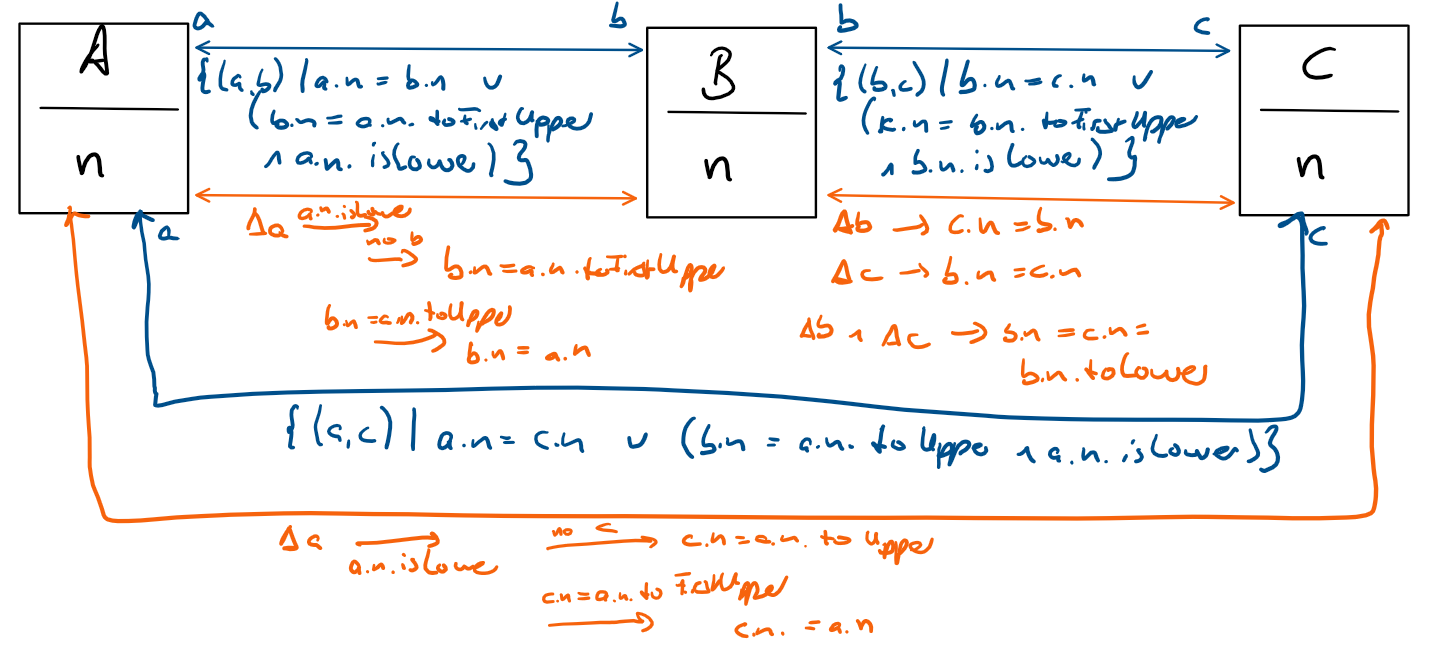
\includegraphics[width=\textwidth]{figures/correctness/orchestration/monotony_counterexample.png}
    \caption{Counterexample for monotony}
    \label{fig:formal:monotonycounterexample}
\end{figure}

One could now argue that there are binary relations in the example, which may never be fulfilled at all. We will later discuss how far relations that cannot be fulfilled should be restricted. However, in general, this is wanted behavior, because in general it may be necessary that transformations produce intermediate states that are not yet consistent with each other. Otherwise this would means that each transformation is always able to directly deliver a state that is consistent to all other relations, which is especially not possible, because other transformations may add further information to the models. More precisely, a relation may consider <a model consistent to all other models that contain any additional information not affected by the transformation. For example, a UML class model may be considered consistent to all Java models with any implementation of the specified methods, thus to an infinite number of models. Now saying that it should not be allowed that the transformation selects one with an empty implementation because that is not consistent to another relations induced by another transformation, such as the relationship to a component model, does not make any sense. Thus having those relation elements that may be considered locally consistent but will never occur in a globally consistent tuple of models does not make sense.
In the example, we can see that such an inconsistent intermediate state is passed through and afterwards a consistent tuple of models is reached if not requiring monotony.
In consequence, requiring monotony from transformations is a too strict requirement, because it is necessary to run through states that may be changed later on.

\begin{theorem}
    An application function for monotone transformations either returns a consistent model or produce a sequence of CPRs returning delta that return models of always growing size (i.e. it diverges).
\end{theorem}

\paragraph{Divergence cannot be avoided}

There are rather equal network, one that terminates after a long time and one that never terminates. 
Consider the example. The relations are defined in a way such that for any allocation for any of them a consistent tuple of models can be found. However, the transformations are not able to find it because they make "bad" choices from a set of choices that are conflicting. 
This can be seen in the example that we have already given in \autoref{fig:correctness:no_execution_order}.

Thus, systematically avoiding divergence is not possible. 

\textbf{Central insight:} Alternation / Divergence cannot be avoided systematically (like in ordinary programming), if not restricting transformations in a way that may not be reasonable.



\subsection{Unresolvability}

Discuss why no execution order may exist although relations are compatible.
If not even an order exists, the application function or the algorithm can, for sure, not find it.

However, we found that we cannot always find an execution order if it exists and we were not able to find restrictions to transformations to ensure that it exists.
We expect the same for the existence of an execution order at all.
All restrictions we can make are likely to be too restrictive.
The problem arises when there is an overlap of consistent models between some transformations, but they always decide for other elements that are not in the overlap of consistent models.
It would, obviously, require the transformation to know about the others to ensure that this is not the case.
This conflicts our assumption.

Finally, it may be valid that for some changes no execution exists, because the change can not be processed on purpose \todo{Give example for that!}.
Should this be the case if we assume compatibility?

Although a more detailed investigation of the claim that we cannot define reasonable requirements to the transformations to ensure that they can always be ordered to restore consistency is a topic for further research, we did not investigate it in the scope of this thesis.
Since we found it necessary to find a conservative algorithm that can deal with the case that no execution is found anyway, that algorithm covers the case that no execution order exists as well and thus is a solution for this problem as well.

Beispiel:
\begin{itemize}
    \item Das ist im allgemeinen aber nicht Fall. Letztendlich trifft jede Transformation lokale Entscheidungen. Beispielsweise könnte jede einzelne Transformation gegeben eine beliebige Änderung immer dieselben Modelle (bzw. Änderungen die dazu führen) zurück liefern (im trivialsten Fall leere Modelle). Dann erfüllt jede Transformation ihre Korrektheitseigenschaft bzgl. ihrer Relation, aber das Netzwerk muss nicht korrekt sein, da bspw. T(A,B) und T(B,C) sich immer für verschiedene Instanzen von B entscheiden. Es gäbe somit nie eine konsistente Lösung für eine beliebige Ausführungsreihenfolge der Transformationen, auch wenn die Relationen das erlauben würden.
    \item Beispiel mit Namen, wo eine Transformation immer den großen Namen zurück liefert, die andere immer den kleinen. T(A,B) bildet A auf gleiches B ab und beide auf kleine Schreibweise, obwohl beide erlaubt sind. Erzeuge A="a", dadurch B="a". T(B,C) bildet B auf C ab und beide auf große Schreibweise, obwohl beide erlaubt sind. Somit macht sie das zu B="A" und C="A". Nun wird T(A,B) wieder beide klein machen usw. Allerdings wäre eine insgesamt valide Lösung einfach alle groß oder alle klein zu machen, aber die Transformationen finden diesen Zustand nicht. 
\end{itemize}



\section{Conservative Orchestration}
Conclude: Conservativeness rather than correctness or achieving optimality (but improving the latter one)

\todo{Remove much of the following}

\mnote{Achieving a correct application function}
The definition of the application function basically ensures that the function either returns $\bot$ or executes the \modellevelconsistencypreservationrules given by the orchestration function to retrieve a changes tuple of models.
It is considered \emph{correct} if it ensures that its result is either $\bot$ or a consistent model tuple by executing the \modellevelconsistencypreservationrules given by the orchestration function.
% A correct application function thus has to ensure that its result is either $\bot$ or a consistent model tuple by executing the \modellevelconsistencypreservationrules given by the orchestration function.
In consequence, the application function can be realized by simply executing the result of the orchestration function and check whether the resulting model tuple is consistent or not and return an appropriate result.
Such a realization is generic and does not depend on the actual consistency preservation rules and orchestration function but represents a generic behavior.
Additionally, this gives an implementation of that function the ability to present a faulty result to the user, which eases finding out why no consistent state was reached.

\mnote{Correctness is not crucial}
Finally, correctness is not crucial, because correctness can easily be achieved by performing any execution of transformations and just ensuring that we terminate at some point in time and then decide whether the resulting models are consistent or not and appropriately deliver the result.

\mnote{How to define an orchestration function that is as optimal as possible?}
The remaining difficulty is how to define an orchestration function that fulfills the definition, i.e., to find a finite sequence of transformations, and also one that improves optimality, as an \emph{optimal} function can never be given.
Although the definition of the orchestration function proposes a closed description of that function, in practice such a function will not have a closed form but will be realized as an algorithm that dynamically decides which transformation to execute next.
Therefore the arising problem is that the length of the sequence to execute is not known a priori. Therefore, we need some abortion criterion. When a consistent result is found, this criterion is easy. But since we do not know whether a sequence exist, we need an abortion criterion that is reasonable and does not cut off the process although a consistent solution could be found, thus reducing optimality.
A simple realization for that algorithm to deliver a finite sequence of transformations would be to define a fixed termination criterion, such as a specific number of transformation executions. However, there is no upper bound for the number of executed transformations necessary to achieve consistency. Still, a fixed number (even 0) could be defined for the number of executed transformations to fulfill the definition. Hence, optimality would be 0 then as a consistent result is never reached. We therefore discuss in the following how to define an appropriate orchestration function and how to optimize it.

\mnote{Achieving a correct application function}
The definition of the application function basically ensures that the function either returns $\bot$ or executes the \modellevelconsistencypreservationrules given by the orchestration function to retrieve a changes tuple of models.
It is considered \emph{correct} if it ensures that its result is either $\bot$ or a consistent model tuple by executing the \modellevelconsistencypreservationrules given by the orchestration function.
% A correct application function thus has to ensure that its result is either $\bot$ or a consistent model tuple by executing the \modellevelconsistencypreservationrules given by the orchestration function.
In consequence, the application function can be realized by simply executing the result of the orchestration function and check whether the resulting model tuple is consistent or not and return an appropriate result.
Such a realization is generic and does not depend on the actual consistency preservation rules and orchestration function but represents a generic behavior.
Additionally, this gives an implementation of that function the ability to present a faulty result to the user, which eases finding out why no consistent state was reached.

\mnote{Correctness is not crucial}
Finally, correctness is not crucial, because correctness can easily be achieved by performing any execution of transformations and just ensuring that we terminate at some point in time and then decide whether the resulting models are consistent or not and appropriately deliver the result.

\mnote{How to define an orchestration function that is as optimal as possible?}
The remaining difficulty is how to define an orchestration function that fulfills the definition, i.e., to find a finite sequence of transformations, and also one that improves optimality, as an \emph{optimal} function can never be given.
Although the definition of the orchestration function proposes a closed description of that function, in practice such a function will not have a closed form but will be realized as an algorithm that dynamically decides which transformation to execute next.
Therefore the arising problem is that the length of the sequence to execute is not known a priori. Therefore, we need some abortion criterion. When a consistent result is found, this criterion is easy. But since we do not know whether a sequence exist, we need an abortion criterion that is reasonable and does not cut off the process although a consistent solution could be found, thus reducing optimality.
A simple realization for that algorithm to deliver a finite sequence of transformations would be to define a fixed termination criterion, such as a specific number of transformation executions. However, there is no upper bound for the number of executed transformations necessary to achieve consistency. Still, a fixed number (even 0) could be defined for the number of executed transformations to fulfill the definition. Hence, optimality would be 0 then as a consistent result is never reached. We therefore discuss in the following how to define an appropriate orchestration function and how to optimize it.

\textbf{Overall Goal:} Find correct orchestration function that improves optimality.

There are two ways to improve optimality of the orchestration function:
\begin{enumerate}
    \item Optimize the orchestration function, i.e., find a good order (probably this is not possible), at least find an order that helps the developer to find problems
    \item Optimize the input, i.e., define requirements to the transformations and their relations representing the input to optimize optimality
\end{enumerate}
\todo{We need an example for that}

Both goes hand in hand, because restrictions to the input can never lead to an orchestration function that always terminates without leading to unsupported relevant cases.

This conform to two approaches:
\begin{enumerate}
    \item Dynamic decision about selected transformation and abortion criteria
    \item Constructive restrictions that ensure that appropriate order is (easily) found
\end{enumerate}

\todo{Application function can be generically defined, orchestration maybe not? We actually want to ensure that both are generic and none of them has to be defined for a specific project.}

\begin{itemize}
    \item We conclude that we need to deal with the situation of undecidability. In consequence, orchestration must operate conservatively, i.e., we cannot assume to always find a solution, but if find it, it must be consistent.
    \item One approach could be to reduce conservativeness. But even if we reduced conservativeness, we would not be able to completely eliminate it and thus have to deal with the situation that the strategy does not find a solution although it may exist.
    \item We thus propose an approach that helps to identify the reason when the strategy is in the conservative case, i.e., not able to find a solution although it exists.
\end{itemize}


\subsection{Reducing Conservativeness}

Due to Turing-completeness of the network this would mean that the orchestration function can decide whether a Turing machine halts, which is proven impossible.
Thus, our only goal can be to achieve optimality as far as possible in terms of reducing the degree of conservativeness, i.e., reduce the cases in which no sequence is found although it exists.

We can define a measure for the optimality of an orchestration function:
\begin{align*}
    &
    Optimality_{\orcfunction{\consistencypreservationruleset{}}} = \frac{\mathtext{\# of model / delta pairs for which the function finds an order that terminate consistently}}{\mathtext{\# of model / delta pairs for which an order that terminates consistently exists}}
\end{align*}

In fact, both these numbers usually infinite, an there is an infinite number of possible models and deltas. However, it does finally not matter for us what the actually value is, but only how to improve that value.
\todo{We have to map that value to compatibility, which reduces the number of potential false orders.}


\subsection{Detecting Alternation and Divergence}

\paragraph{Detecting Alternation / Divergence}

In consequence, we propose to dynamically deal with alternation / divergence.
To detect alternations, the execution can simply track if a state way already processed. Apart from spatial problems, this does always work.
Finding divergence is not that easy, because it is generally not possible to define an upper bound for the number of executions of a single transformation.
This is due to the reason that, again, this conflicts with the Halting problem.
We can see this at the simple example in \autoref{fig:formal:noupperboundexample}.

\begin{figure}
    \centering
    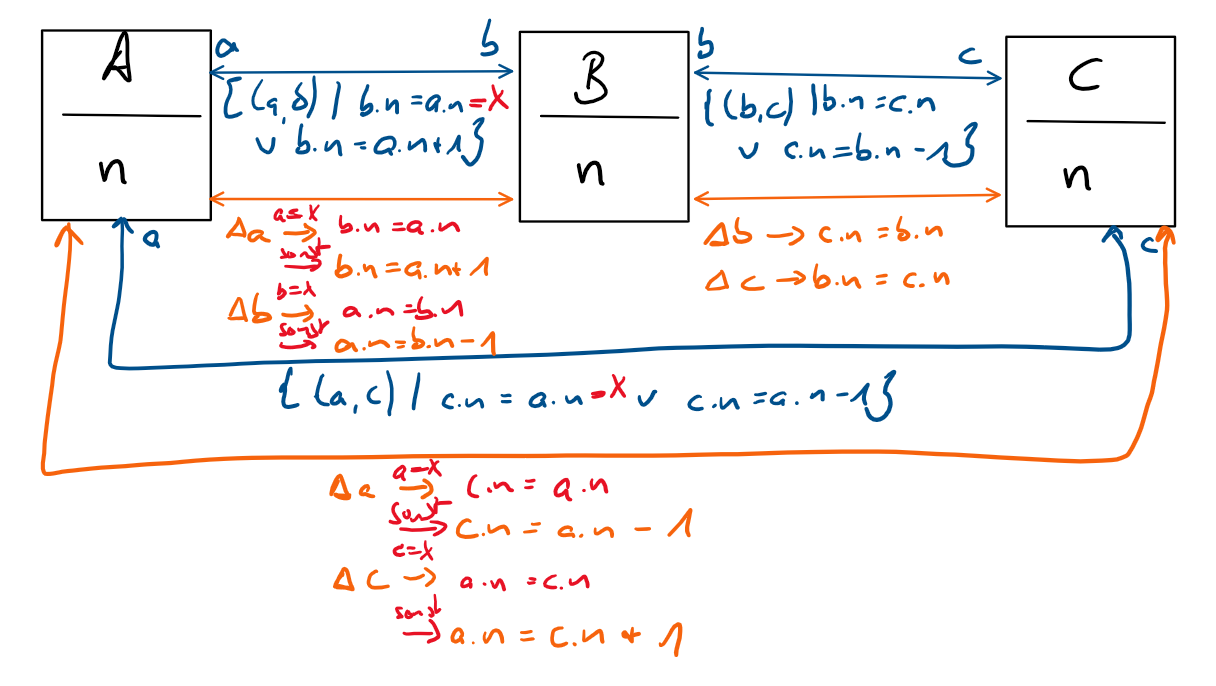
\includegraphics[width=\textwidth]{figures/correctness/orchestration/no_upper_bound_example_old.png}
    \caption{Example for no upper bound}
    \label{fig:formal:noupperboundexample}
\end{figure}

Depending on the value X, the transformations have to be executed X times to result in a consistent state. This value can be arbitrarily chosen, thus an arbitrary number of executions may be necessary to terminate in a consistent state.

\todo{Moved from single execution section -> revise}
\begin{theorem}[Orchestration with Unbounded Executions]
    \label{theorem:unbounded_execution}
    For any set of transformations $\transformationset{T}$, there can be models $\modeltuple{m}$ and changes $\changetuple{}$ to them for which each possible orchestration function $\orcfunction{\transformationset{T}}$ with whom $\appfunction{\orcfunction{\transformationset{T}}}(\modeltuple{m}, \changetuple{})$ is consistent, such that $\abs{\orcfunction{\transformationset{T}}(\modeltuple{m}, \changetuple{})} > \abs{\transformationset{T}}$.
\end{theorem}
\begin{proof}
    We know from \autoref{lemma:minimal_executions} that $\transformationset{T}_{inc}$ requires at least $4$ executions of $\transformation{T}_{12}$ for the inputs defined in \autoref{lemma:minimal_executions} when selecting $x \geq 5$.
    Thus, for any orchestration function, we know that $\abs{\orcfunction{\transformationset{T}}(\modeltuple{m}, \changetuple{})} > 4 > 3 = \abs{\transformationset{T}_{inc}}$.
    This proves the theorem by example.
\end{proof}

From an engineering perspective, this is still unwanted behavior. We claim that a transformation network that takes thousands of executions of the same transformation to find a consistent state works not as expected and if running into a failure would expose severe problems to find the reasons for that failures.
Thus, we propose to simply abort the execution after some time to be sure not to run in an endless loop.

Finally, this problem is comparable to ordinary programming, because there the same situations regarding alternation and divergence can occur that result in non-termination of a program.
As we all know, it is impossible to systematically avoid that, but just possible to carefully develop the program and apply best practices to avoid such situations.


\textbf{Conclusion:} We cannot systematically improve optimality / reduce conservativeness and also not dynamically terminate when divergence is detected. Especially, there is no guarantee wo when also alternation is detected. There can be an arbitrary high number of execution before alternation is detected.
Thus, we propose an algorithm that terminates deterministically and returns $\bot$ also when it is not able to find a solution in a fixed number of steps, but improves the ability for the transformation developer or user to find out why in specific situation no solution can be found.




\section{A Conservative Application Algorithm}

Propose Provenance and Reactions Strategy.




\section{Summary}

%\todo{Property for orchestration: if no consistent solution found then there is no further transformation that could be executed without alternation or because no transforamtion is applicable (undefined for current state, e.g. because of monotony)}


\begin{insight}[Orchestration]
    We have proven that orchestration of modular and independently developed transformations is undecidable without restrictions to the individual transformations.
    We found that there are no reasonable restrictions to the individual transformations that make orchestration decidable.
    In consequence, transformation orchestration needs to be conservative.
    In addition to reducing conservativeness, it can be useful to find an orchestration strategy that supports developers and users of transformation to find the reason for a transformation network not finding a consistent result after certain changes.
    One such strategy is given by inductively restoring consistency for subsets of the transformations and thus improving reasoning about provenance whenever consistency cannot be restored.
\end{insight}




\section{Old Notes}

%\section{Restrictions vs. Conservativeness}

\todo{First restriction: Input delta of APP only contains changes to one model -> no synchronisation}
\todo{Second restriction: Input delta is not rejected}
\todo{Third restriction: Generated deltas are monotone}

% From a theoretical perspective, it is always possible to a specify consistency relations according to the definition, as it is just a subset of elements.
% It is also always possible to define a consistency preservation rule for a consistency relation according to its definition, as can simply return any any element of the relation.
% \todo{This is not true: the source model may not be in the relation, then its not possible, at least with the current definition. With a synchronizing transformation, any modification can be made to both models, then its fine.}
% The generalization function is generic, so it can always be applied.
% Finally, the consistency preservation application function is an artifact that cannot be easily specified according to the definition for a given set of consistency preservation rules.
% It is always possible to have a set of consistency preservation rules for which no application function can be defined that returns a consistent result for at least one input model and change tuple, as there is not sequence of consistency preservation rules that achieves that.
% \todo{Example!}
% Even worse, the problem to define such a function is Turing-complete, which makes it impossible to decide whether such a function exists.
% \todo{Show Turing-completeness}
% Consequence: From a theoretical perspective, this function is the crucial part!

% Essential problem: One transformation may restore consistency between A and B and another between A and C. If then a transformation restores consistency between B and C, the resulting B' and C' may not be consistent A anymore.

% Alternative to an app function: Define a \emph{well-definedness} property for a set of transformations, requiring that they can be executed in any order to always terminate consistently. However, this is a very strict requirement, which can usually not be fulfilled, so we do not further investigate that.
% \todo{Give simple example why that does not work.}


% Best-behaved app function: Whenever there is a sequence of CPRs, the app function finds item. This is still not possible due to Turing-completeness. The function would need to decide whether the network terminates or not.

% Only achievable app function is a best-effort (i.e. conservative) function: A function that either returns a consistent set of models or that does return bottom. Not making a statement about how often a correct result is returned in comparison to how often it is possible.

% This approach is conservative. The question is then, how high the degree of conservativeness is. In the worst case, a function that always returns bottom would fulfill the definition, but that is not what we want. We want to reduce conservativeness.

% Goal: Find a solution in as many cases as possible, abort in the others (conservatively). There are two subgoals to achieve that:
% 1. Function must be correct, i.e. always terminate (no endless sequence of CPR) and terminate in a consistent state
% 2. Function must be as less conservative as possible

% It is clear that we cannot give a closed function for APP that just by a given change returns a sequence of CPR that results in a consistent state. APP has to be calculated dynamically during execution. Therefore we consider it as an algorithm in the following.

Annahmen:
\begin{itemize}
    \item Nutzeränderungen dürfen nicht rückgängig gemacht werden.
    \item Nutzeränderungen lassen sich so feingranular zerlegen, dass, falls durch die Erzeugung/Änderung eine Konsistenzrelation verletzt wird, es in jeder unabhängigen Teilmenge von Konsistenzrelationen eine verletzte Konsistenzrelation gibt, für die die geänderten Elemente einem Condition Elemente entsprechen, es also insbesondere keine Teilmenge der geänderten Element gibt, die bereits dieses Condition Element sind. Ansonsten ist durch unsere Kompatibilitäts-Definition nicht sichergestellt, dass eine konsistente Modellmenge gefunden werden kann.
\end{itemize}




% \section{Considerations}

% Zu diskutierende Dinge:
% \begin{itemize}
%     \item Im Allgemeinen könnte eine Transformation beliebige dieser Deltasequenzen modifizieren. Wir verlangen jedoch, dass eine Transformation nur Deltas anhängt, also die Sequenzen länger werden
%     \item Genauer beschränken wir auch, welche Sequenzen eine Transformation sehen und ändern darf, genau gesagt darf sie die Sequenzen von zwei Modellen sehen und eine davon verlängern.
%     \item Hier kommt bereits der Unterschied zu bisherigen Transformationen, denn die sehen nur Deltas an einem Modell und erzeugen Deltas an dem anderen. Das ist bei uns schon gänzlich anders. Bidirektionale Transformationen unterstützen das im Übrigen auch nicht, sondern sind nur Spezifikationen, aus denen sich Wiederherstellungsroutinen für beide Richtungen ableiten lassen (siehe Stevens 2010)
% \end{itemize}


% Trivialisierung des Problems:
% \begin{itemize}
%     \item Ohne weitere Annahmen ist das immer dadurch erreichbar, dass die Transformationen einen beliebigen anderen Zustand der Modelle produzieren. Im einfachsten Fall liefert jede Transformation immer die gleichen konsistenten Modelle zurück, unabhängig von der Änderung. Dann ist der Endzustand der Modelle nach der Ausführung des Netzwerks immer der gleiche.
%     \item Das ist im allgemeinen aber nicht Fall. Letztendlich trifft jede Transformation lokale Entscheidungen. Beispielsweise könnte jede einzelne Transformation gegeben eine beliebige Änderung immer dieselben Modelle (bzw. Änderungen die dazu führen) zurückliefern (im trivialsten Fall leere Modelle). Dann erfüllt jede Transformation ihre Korrektheitseigenschaft bzgl. ihrer Relation, aber das Netzwerk muss nicht korrekt sein, da bspw. T(A,B) und T(B,C) sich immer für verschiedene Instanzen von B entscheiden. Es gäbe somit nie eine konsistente Lösung für eine beliebige Ausführungsreihenfolge der Transformationen, auch wenn die Relationen das erlauben würden.
%     \item Beispiel mit Namen, wo eine Transformation immer den großen Namen zurückliefert, die andere immer den kleinen. T(A,B) bildet A auf gleiches B ab und beide auf kleine Schreibweise, obwohl beide erlaubt sind. Erzeuge A="a", dadurch B="a". T(B,C) bildet B auf C ab und beide auf große Schreibweise, obwohl beide erlaubt sind. Somit macht sie das zu B="A" und C="A". Nun wird T(A,B) wieder beide klein machen usw. Allerdings wäre eine insgesamt valide Lösung einfach alle groß oder alle klein zu machen, aber die Transformationen finden diesen Zustand nicht. 
%     \item Allgemeiner ist zu sagen, dass ein Transformationsnetzwerk eine Turing-Maschine emulieren kann. \todo{Nachweisen!}
%     Im allgemeinen terminiert das Netzwerk somit nicht, schlimmer noch, es ist unentscheidbar, ob das Netzwerk hält (siehe Halteproblem).
%     \item Dies zeigt bereits, dass keine Ausführungsfunktion definiert werden kann, die immer ein konsistentes Ergebnis liefert.
%     \item Wir versuchen daher Annahmen an Transformationen zu finden, um diese Fälle auszuschließen bzw. systematisch zu verringern. 
%     \item Außerdem möchten wir eine Ausführungsfunktion haben, die ein konsistentes Ergebnis liefert oder einen Fehler, denn es muss nicht immer eine korrekte Lösung geben. Ziel ist es dann die Anzahl der Fälle, in denen sie einen Fehler zurückgibt, zu reduzieren.
% \end{itemize}


% Zielsetzung:
% \begin{itemize}
%     \item Korrekte Anwendungsfunktion finden (in bestehenden Arbeiten~\cite{stevens2017a}) auch "Resolution" genannt (formal definieren!):
%     \item Welche Anforderungen müssen wir dafür an die Transformationen stellen, damit solch eine Funktion definiert werden kann?
%     \item Wir bezeichnen das Transformationsnetzwerk, in dem eine Transformation eingesetzt wird, als "Kontext"
%     \item Welche dieser Eigenschaften kann die einzelne Transformation (ohne Kenntnis der anderen) erfüllen und für welche muss der Kontext (d.h. die anderen Transformationen) bekannt sein?
%     \item $\Rightarrow$ Interesse an "kontextfreien" Eigenschaften (lassen sich ohne Kenntnis der anderen Transformationen sicherstellen -> Wiederverwendbarkeit) und "kontextsensitiven" Eigenschaften (Erfüllung der Eigenschaft nur durch Kenntnis über das Transformationsnetzwerk möglich)
%     \item Kontextfreie Eigenschaften involvieren solche, die wir eh schon von Transformationen kennen (Korrektheit einer Transformation, Hippokratie etc.) und solche, die dadurch zustande kommen, dass man weiß, dass diese Transformation in einem Netzwerk eingesetzt werden soll.
%     \item Zielsetzungsoptionen:
%     \begin{itemize}
%         \item Wir schränken die Transformationen so ein, dass es immer mindestens eine Ausführungsreihenfolge der Transformationen gibt, sodass für jede beliebige Änderung ein konsistentes Ergebnis durch Anwenden der Transformationen gefunden werden kann
%         \item Wir akzeptieren, dass es Änderungen gibt, für die das Netzwerk kein konsistentes Ergebnis produzieren kann. Dann muss das Netzwerk (mindestens) in diesen Fällen mit einer Fehlermeldung terminieren.
%         \item Eine Option ist, dass das Netzwerk dieses Verhalten nur approximiert bzw. approximieren kann, dann muss es sich konservativ verhalten, d.h. im Fall, dass es keine Lösung gibt, auf jeden Fall eine Fehlermeldung geben, und im Fall, in dem es eine Lösung gibt, diese bestenfalls finden oder ausgeben, dass es keine finden kann (d.h. keine False Positives bzw. Nicht-Terminierung). Ziel ist es dann den Grad der Konservativität zu minimieren.
%     \end{itemize}
%     \item Lösungsoptionen (Grad der Einschränkung an die Transformationen):
%     \begin{itemize}
%         \item Hohe Einschränkung: Jede beliebige Reihenfolge von ausgeführten Transformationen führt letztendlich zu einem korrekten Ergebnis (Fixpunktiteration -- Allquantifizierung) -- Hippokratie-Eigenschaft sorgt dafür, dass keine Transformation wieder etwas ändert, wenn Konsistenz bereits hergestellt ist.
%         Diese Eigenschaft ist in der Praxis möglicherweise zu strikt, da sie sehr starke Anforderungen an die Transformationen stellen müsste. Dafür wäre aber die Anwendungsfunktion trivial.
%         \item Mittlere Einschränkung: Es gibt eine Reihenfolge von ausgeführten Transformationen für jede Änderung die terminiert (Existenzquantifizierung) und die Ausführungsfunktion findet diese Reihenfolge.
%         Utopisch, dass die Anwendungsfunktion aus (potentiell sehr mächtigen) Transformationen die richtige Reihenfolge errechnen kann. Dafür aber (möglicherweise) weniger Anforderungen an die Transformationen (zumindest nicht mehr Anforderungen, denn die Allquantifzierung induziert die Existenzquantifizierung). Eine Funktion könnte dann zumindest nach best-effort versuchen, die richtige Reihenfolge zu finden und konservativ abbrechen, wenn sie diese nicht finden kann (also entweder konsistent terminieren oder terminieren mit der Aussage, dass es entweder keine solche Reihenfolge gibt -- bei relaxierten Anforderungen -- oder dass es sie nicht finden kann).  
%         \item Geringe Einschränkung: Es gibt potentiell keine Reihenfolge der Transformationen, die bei einer Änderung zu einer konsistenten Lösung kommt. Hier müsste die Ausführungsfunktion entsprechend einen Fehler ausgeben.
%         \item Bestehende Arbeiten (\cite{stevens2017a}) schlagen auch vor eine Baumstruktur zu berechnen (Spannbaum), in dem nur entlang der Baumkanten die Transformationen ausgeführt werden. Dies ist jedoch eine starke Einschränkung daran, was die Transformationen ausdrücken können. Betrachtet man beispielsweise PCM, UML und Java, und hat eine Änderung in PCM. Dann könnte der Spannbaum entweder PCM -> UML -> Java sein, oder PCM -> UML + PCM -> Java. In ersterem Fall würde Verhaltensbeschreibung, die von PCM nach Java übertragen, aber in UML nicht dargestellt wird, nicht übertragen. Im zweiten Fall würde zusätzliche Information zwischen UML und Java nicht propagiert (Beispiel?) --> Hier sollte auf das Properties-Kapitel verwiesen werden, wo diese "Bottlenecks" erklärt sein sollten, inklusive einem Beispiel, die allgemein Baumstrukturen für Transformationsnetwerke ausschließen.
%     \end{itemize}
%     \item Dies setzt voraus, dass die Transformationen und die Anwendungsfunktion mit jeder beliebigen Nutzer-Änderung umgehen kann. Man kann jedoch auch verlangen, dass die Anwendungsfunktion genau dann, wenn es überhaupt eine Ausführungsreihenfolge gibt, diese findet, und sonst einen Fehler ausgibt.
%     \item \textbf{Wichtig:} Im Allgemeinen kann eine Ausführungsfunktion keine terminierende Reihenfolge berechnen, da die Transformationen Turing-vollständig sind und deshalb die Frage, welche Reihenfolge zu einer Terminierung führt, unentscheidbar ist (Halteproblem). Daher können wir nur einen konservativen Algorithmus angeben, der ein sinnvolles Abbruchkriterium definiert, mit dem die Ausführung beendet wird, auch wenn potentiell eine Lösung hätte gefunden werden können. Die Fragestellung ist also, wie die Ausführungsfunktion aussehen muss, damit sie in möglichst vielen Fällen, in denen es eine terminierenden Reihenfolge gibt, diese auch findet. Insbesondere lässt sich somit keine geschlossene Form für die Ausführungsfunktion angeben, sondern nur ein Algorithmus, der zur Laufzeit eine Reihenfolge (dynamisch) festlegt.
% \end{itemize}





% Notwendigkeit Transformationen oder Anwendungsfunktion einzuschränken:
% \begin{itemize}
%     \item Zeigen, dass es Beispiele gibt, in denen es keine einzige Ausführungsreihenfolge gibt (All-Quantifizierung), die zu einem konsistenten Ergebnis führt:
%     \item Zeigen, dass es Beispiele gibt, in denen es unabhängig von der Ausführungsreihenfolge immer zu einer Alternierung kommt
%     \item Zeigen, dass es Beispiele gibt, in denen es unabhängig von der Ausführungsreihenfolge immer zu einer Divergenz kommt.
%     \item Die Beispiele sollten zeigen, dass wir keine Einschränkungen an die Transformationen machen können, was das Problem aushebelt. D.h. egal welche Einschränkungen ich an die Transformationen definiere, es lassen sich immer Beispiele konstruieren, in denen es keine Ausführungsreihenfolge gibt, in denen sie terminieren.
%     \item Mathematisch zeigen, dass Alternierung und Divergenz die einzigen Probleme sind. D.h. wenn nicht der gleiche Zustand mehrmals durchlaufen wird (Alternierung) und es nicht unendlich viele Zustände gibt (Divergenz), dann ist die Folge endlich.
%     \item Außerdem mathematisch die Abbildung von Transformationen auf Turing-Maschinen zeigen und damit ableiten, dass allgemeine Netzwerke erstmal nicht terminieren müssen (Abbildung auf Halteproblem)
% \end{itemize}

% Zielsetzung die Zweite:
% \begin{itemize}
%     \item Wir definieren möglichst minimale Beschränkungen, die dazu führen, dass das Netzwerk terminiert. D.h. es terminiert entweder konsistent oder es terminiert mit einem Fehler, der sagt, dass entweder keine Konsistenz hergestellt werden kann (es gibt keine Ausführungsreihenfolge der Transformationen, die zu Konsistenz führt) oder dass die Anwendungsfunktion nicht in der Lage war eine passende Ausführungsreihenfolge zu finden (Konservativität)
%     \item Zwei Arten von Beschränkungen
%     \begin{itemize}
%         \item Beschränkungen an die Transformationen, die dazu führen, dass es in mehr Fällen mindestens eine Ausführungsreihenfolge gibt, in der das Netzwerk konsistent terminiert
%         \item Beschränkungen an die Ausführungsfunktion, sodass die Ausführung auf jeden Fall terminiert, wenn auch konservativ, d.h. mit Fehler, obwohl es eine korrekte Lösung gegeben hätte.
%     \end{itemize}
% \end{itemize}



Exkurs: Menge (konsistenter) Modelle bildet keinen topologischen Raum
\begin{itemize}
    \item Topologischer Raum besteht aus Grundmenge und Mengensystem von Teilmengen mit den Eigenschaften, dass die Grundmenge offen ist, der Schnitt endlich vieler Mengen offen und die Vereinigung beliebig vieler Mengen offen ist. 
    \item Die Grundmenge wäre die Menge aller Modellelemente
    \item Diese Menge ist normalweise offen, da z.B. für ein Element mit einem String-Attributwert immer noch das Element mit dem gleichen String-Attributwert plus einem weiteren Symbol in der Menge liegt (und man die Ordnung in der Menge entsprechend definiert). Dass ein Metamodell möglicherweise Einschränkungen definiert und dann im schlimmsten Fall nur ein einziges Modell valide ist, lassen wir hier außen vor.
    \item Betrachten wir nun eine Topologie auf dieser Menge, also ein Mengensystem aus konsistenten Modellen. Leider ist jedoch der Schnitt zweier konsistenter Modelle nicht zwangsläufig konsistent. Insbesondere sind diese Mengen auch nicht offen, da sie die abgeschlossene Menge darstellen, die genau ein Modell beschreiben. 
    \item Somit lässt sich die Definition von Topologien hier nicht anwenden.
\end{itemize}



% \section{No Execution Order with Consistent Result}

% It is obvious that we can define consistency preservation rules for which the orchestration function cannot find an execution order that returns a consistent tuple of models after certain changes. We already gave an example in \autoref{fig:correctness:no_execution_order}. There exists no execution order for any input value that terminates. The transformations will always increase the value, although the defined relations could be fulfilled for the input value, but the transformations never find that solution.

% Although we will discuss restrictions to relations and transformations that reduce the chance that no solution can be found, it will not be possible to ensure that such a solution can always be found. This is due to the reason that transformations can perform arbitrary changes given that transformations are Turing complete, which should not be restricted, because it is unclear which restrictions could be made without forbidding scenarios that should actually we supported. Thus, we assume that transformations are Turing complete.

% We explicitly allow the orchestration function to return a sequence that will, if applied to models and changes to them, not deliver a consistent tuple of models. As discusses, this is supposed to reflect cases in which no such sequence can be calculated.
% However, it may be useful to have some notion of \emph{optimality} that ensures that if a sequence that delivers a consistent result exists, the orchestration function is supposed to find it.
% Formally, this notion looks as follows.

% \begin{definition}[Optimal Consistency Preservation Orchestration Function]
%     \todo{Needs to be adapted to transformations rather than CPRs}
%     Let $\consistencypreservationruleset{}$ be a set of consistency preservation rules for a set of consistency relations $\consistencyrelationset{CR}$ on metamodels $\metamodeltuple{M} = \tupled{\metamodelsequence{M}{n}}$.
%     We say that an orchestration function $\orcfunction{\consistencypreservationruleset{}}$ for these rules is \emph{optimal} if it always returns a sequence that delivers a consistent set of models if possible, i.e.,
%     \begin{align*}
%         &
%         \forall \modeltuple{m} \in \metamodeltupleinstanceset{M} : \forall \changetuple{\metamodeltuple{M}} = \tupled{\change{\metamodel{M}{1}}, \dots, \change{\metamodel{M}{n}}} \in \changeuniverse{\metamodeltuple{M}} :
%         \modeltuple{m} \consistenttomath \consistencyrelationset{CR} \Rightarrow \\
%         & \formulaskip
%         \bigl[ \bigl(
%             \exists \consistencypreservationrule{1}, \dots, \consistencypreservationrule{m} \in \consistencypreservationruleset{} : 
%             \exists \changetuple{\metamodeltuple{M}}' = \tupled{\change{\metamodel{M}{1}}', \dots, \change{\metamodel{M}{n}}'} \in \changeuniverse{\metamodeltuple{M}} :\\
%             & \formulaskip \formulaskip
%             \generalizationfunction{\consistencypreservationrule{1}} \concatfunction \dots \concatfunction \generalizationfunction{\consistencypreservationrule{m}}(\modeltuple{m}, \changetuple{\metamodeltuple{M}}) = (\modeltuple{m}, \changetuple{\metamodeltuple{M}}')\\
%             & \formulaskip \formulaskip
%             \land \tupled{\change{\metamodel{M}{1}}'(\model{m}{1}), \dots, \change{\metamodel{M}{n}}'(\model{m}{n})} \consistenttomath \consistencyrelationset{CR} \bigr) \\
%             & \formulaskip
%             \Rightarrow \bigl(        
%             \exists \consistencypreservationrule{1}', \dots, \consistencypreservationrule{m}' \in \consistencypreservationruleset{} : 
%             \exists \changetuple{\metamodeltuple{M}}'' = \tupled{\change{\metamodel{M}{1}}'', \dots, \change{\metamodel{M}{n}}''} \in \changeuniverse{\metamodeltuple{M}} :\\
%             & \formulaskip \formulaskip
%             \orcfunction{\consistencypreservationruleset{}}(\modeltuple{m}, \changetuple{\metamodeltuple{M}}) = \tupled{\consistencypreservationrule{1}', \dots, \consistencypreservationrule{m}'} \\
%             & \formulaskip \formulaskip
%             \land \generalizationfunction{\consistencypreservationrule{1}'} \concatfunction \dots \concatfunction \generalizationfunction{\consistencypreservationrule{m}'}(\modeltuple{m}, \changetuple{\metamodeltuple{M}}) = (\modeltuple{m}, \changetuple{\metamodeltuple{M}}'')\\
%             & \formulaskip \formulaskip
%             \land \tupled{\change{\metamodel{M}{1}}''(\model{m}{1}), \dots, \change{\metamodel{M}{n}}''(\model{m}{n})} \consistenttomath \consistencyrelationset{CR}
%         \bigr) \bigr]
%     \end{align*}
% \end{definition}

% Unfortunately, optimality is a property that we cannot request from an orchestration function. Optimality would mean that the orchestration function can decide whether there is sequence of transformations that leads to consistent models and thus terminate.
% Due to Turing-completeness of the network this would mean that the orchestration function can decide whether a Turing machine halts, which is proven impossible.
% Thus, our only goal can be to achieve optimality as far as possible in terms of reducing the degree of conservativeness, i.e., reduce the cases in which no sequence is found although it exists.

% We can define a measure for the optimality of an orchestration function:
% \begin{align*}
%     &
%     Optimality_{\orcfunction{\consistencypreservationruleset{}}} = \frac{\mathtext{\# of model / delta pairs for which the function finds an order that terminate consistently}}{\mathtext{\# of model / delta pairs for which an order that terminates consistently exists}}
% \end{align*}

% In fact, both these numbers usually infinite, an there is an infinite number of possible models and deltas. However, it does finally not matter for us what the actually value is, but only how to improve that value.
% \todo{We have to map that value to compatibility, which reduces the number of potential false orders.}



% \subsection{Achieving an Always Correct Application Function}
% % This discusses the case that the application function is optimal
% \todo{These problem cannot occur if a function fulfills the definition, because it always finds a sequence. So the question is how to fulfill the definition.}

% It is easy to achieve that the APP function only terminates in a consistent state, because knowing the relations allows to check whether all relations are fulfilled. 
% \todo{Need to define that a transformation may not be able to process a specific change? Then there could be inconsistent terminiation because a transformation cannot be executed anymore.}

% Problems due to which the function does not terminate: Alternation and Divergence

% Alternation: Run through same state twice
% Divergence: Always produce new states without reaching a consistent state

% Two possibilities to avoid problems:
% 1. Make assumptions to transformations that avoid them
% 2. Detect them dynamically and abort


% \subsubsection{Avoiding Alternation / Divergence}

% Making assumptions that avoid them is rather hard, as we will show in the following.

% \paragraph{Idea:} Require monotony to avoid alternation

% We would have to relax the definition of transformation to be monotone, because if a transformation is monotone, it may only append information, but this is not always possible, as can be seen in the following example. A monotone transformation must be able to return bottom if it cannot make further changes to restore consistency to the relation.

% \begin{definition}[Monotone Transformation]
%     Transformation gets models M and deltas D and produces new deltas D'. Taking the union of the original models M and the new models D'(M), then D(M) must be a subset of that, because other elements would have been added and removed afterwards or elements would have been changes once by D and again in a different way by D'.

%     Generally, monotony could also mean that only the same complete model state is not passed twice. \todo{Why dont we do that?}
% \end{definition}

% This would mean that each transformation only appends changes, i.e., if an element was added/removed, the transformation may not do the inverse. The same applies to attribute/reference changes: if an attribute/reference was already changes it may not be changed again.
% This way, it is by design impossible to pass through the same state again. Actually, if a monotone transformation returns bottom, the network has to terminate with a failure.
% However, this is hard restriction to transformations. It leads to the fact that in some networks that actually have a simple solution no solution is found at all. This can be easily seen at the example in \autoref{fig:formal:monotonycounterexample}. In the example adding "aa" to the left model, any execution order of the transformations leads to the situation that a previous change must be revoked to result in a consistent state. However, it is possible to derive a consistent state for that input change.

% \begin{figure}
%     \centering
%     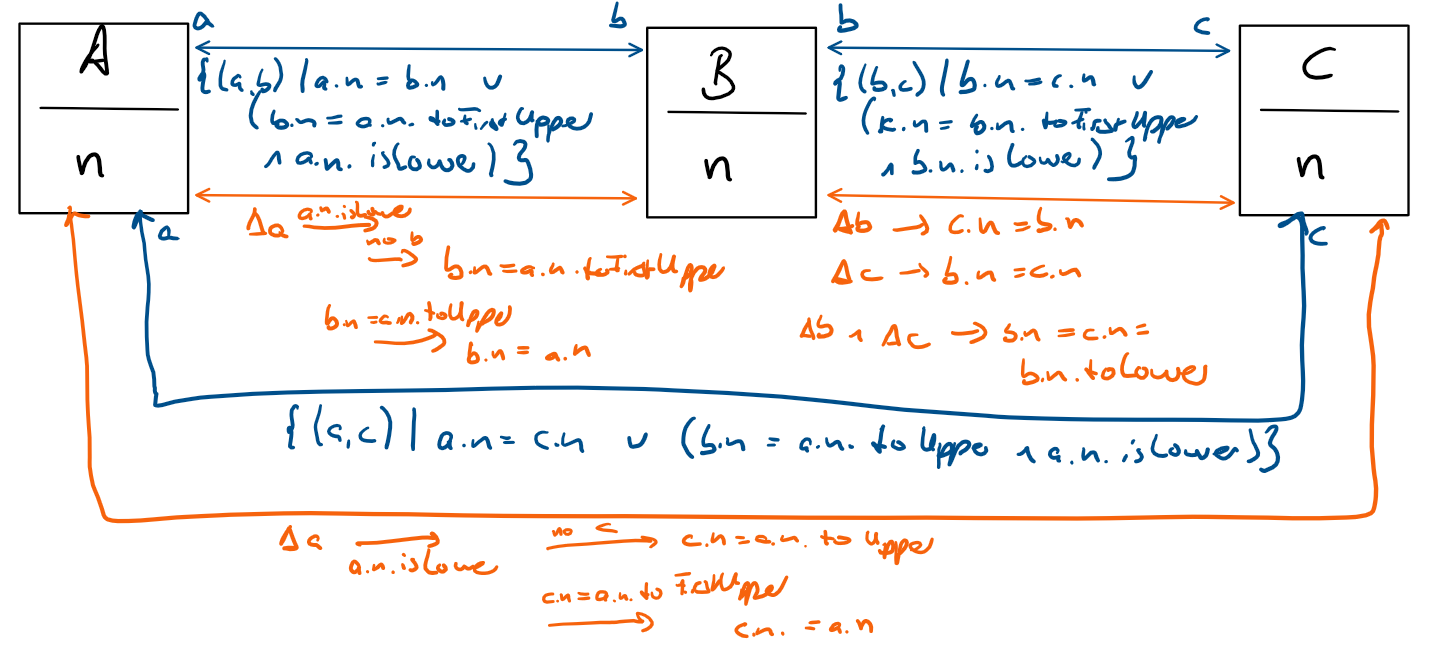
\includegraphics[width=\textwidth]{figures/correctness/orchestration/monotony_counterexample.png}
%     \caption{Counterexample for monotony}
%     \label{fig:formal:monotonycounterexample}
% \end{figure}

% One could now argue that there are binary relations in the example, which may never be fulfilled at all. We will later discuss how far relations that cannot be fulfilled should be restricted. However, in general, this is wanted behavior, because in general it may be necessary that transformations produce intermediate states that are not yet consistent with each other. Otherwise this would means that each transformation is always able to directly deliver a state that is consistent to all other relations, which is especially not possible, because other transformations may add further information to the models. More precisely, a relation may consider <a model consistent to all other models that contain any additional information not affected by the transformation. For example, a UML class model may be considered consistent to all Java models with any implementation of the specified methods, thus to an infinite number of models. Now saying that it should not be allowed that the transformation selects one with an empty implementation because that is not consistent to another relations induced by another transformation, such as the relationship to a component model, does not make any sense. Thus having those relation elements that may be considered locally consistent but will never occur in a globally consistent tuple of models does not make sense.
% In the example, we can see that such an inconsistent intermediate state is passed through and afterwards a consistent tuple of models is reached if not requiring monotony.
% In consequence, requiring monotony from transformations is a too strict requirement, because it is necessary to run through states that may be changed later on.

% \begin{theorem}
%     An application function for monotone transformations either returns a consistent model or produce a sequence of CPRs returning delta that return models of always growing size (i.e. it diverges).
% \end{theorem}


% \paragraph{Divergence cannot be avoided}

% There are rather equal network, one that terminates after a long time and one that never terminates. 
% Consider the example. The relations are defined in a way such that for any allocation for any of them a consistent tuple of models can be found. However, the transformations are not able to find it because they make "bad" choices from a set of choices that are conflicting. 
% This can be seen in the example that we have already given in \autoref{fig:correctness:no_execution_order}.

% Thus, systematically avoiding divergence is not possible. 



% \paragraph{Detecting Alternation / Divergence}

% In consequence, we propose to dynamically deal with alternation / divergence.
% To detect alternations, the execution can simply track if a state way already processed. Apart from spatial problems, this does always work.
% Finding divergence is not that easy, because it is generally not possible to define an upper bound for the number of executions of a single transformation.
% This is due to the reason that, again, this conflicts with the Halting problem.
% We can see this at the simple example in \autoref{fig:formal:noupperboundexample}.

% \begin{figure}
%     \centering
%     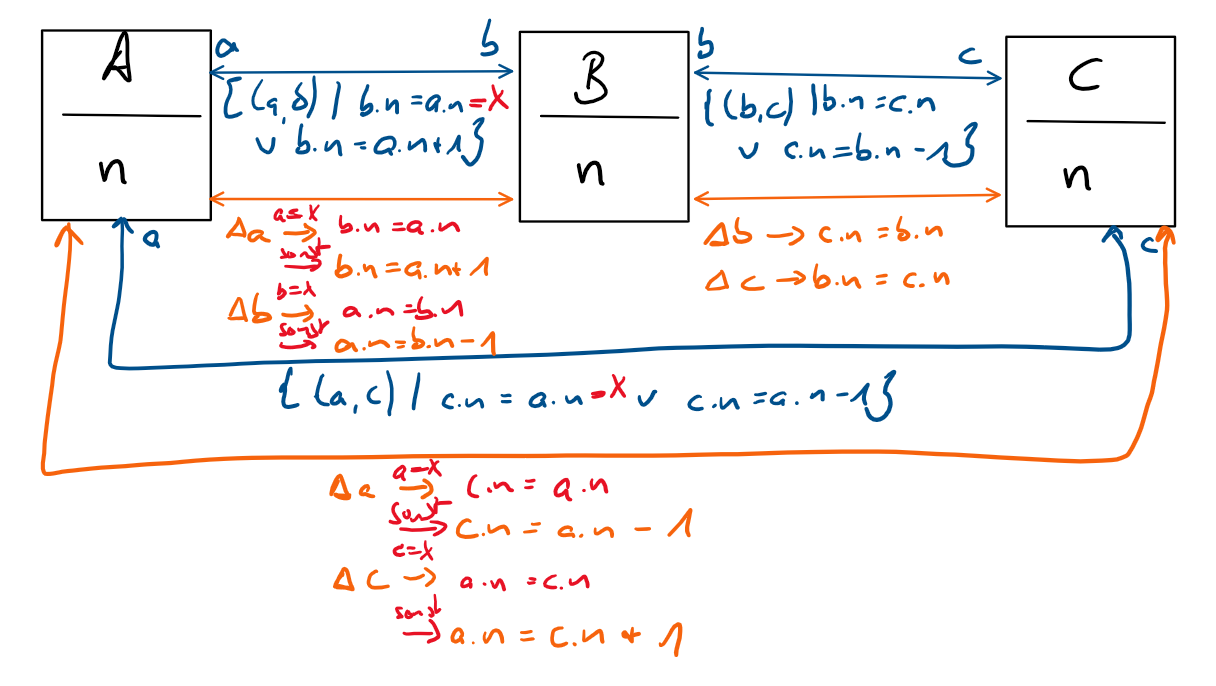
\includegraphics[width=\textwidth]{figures/correctness/orchestration/no_upper_bound_example.png}
%     \caption{Example for no upper bound}
%     \label{fig:formal:noupperboundexample}
% \end{figure}

% Depending on the value X, the transformations have to be executed X times to result in a consistent state. This value can be arbitrarily chosen, thus an arbitrary number of executions may be necessary to terminate in a consistent state.

% From an engineering perspective, this is still unwanted behavior. We claim that a transformation network that takes thousands of executions of the same transformation to find a consistent state works not as expected and if running into a failure would expose severe problems to find the reasons for that failures.
% Thus, we propose to simply abort the execution after some time to be sure not to run in an endless loop.

% Finally, this problem is comparable to ordinary programming, because there the same situations regarding alternation and divergence can occur that result in non-termination of a program.
% As we all know, it is impossible to systematically avoid that, but just possible to carefully develop the program and apply best practices to avoid such situations.

% In the following, we propose measures to reduce the number of cases in which problematic cases can occur.
% In a case study, we will see that using such measures already resolves most of the problems that can occur.
% Additionally, we propose an orchestration strategy that improves the possibility to find errors in case something goes wrong.

% \textbf{Central insight:} Alternation / Divergence cannot be avoided systematically (like in ordinary programming), if not restricting transformations in a way that may not be reasonable.

% \subsection{Reducing Conservativeness of the Application Function}

% Goal: Find a solution in as many cases as possible, abort in the others (conservatively). There are two approaches to achieve that: 
% 1. Reduce the number of cases in which there is no solution by adding assumptions to the relations and transformations (restrict input of app function)
% 2. Improve the ability to find a solution if it exists (improve capabilities of app function)
% Secondary goal: In cases, in which no solution is found, support the user in understanding why no solution was found.


% Regarding 1: Reduce problematic cases


% 1. reduce cases in which there is no such solution
% 1.1. On relation level: Only sets, so analysis possible.
% Ensure that relations are defined in a way such that they do not allow a locally correct set of CPRs that has no APP solution. If there is a pair of models (or elements of a fine-grained relation) in a relation, a CPR may return it. But if there is no consistent tuple of models containing these two, it does not make any sense to consider these elements (even worse, if we have monotony, adding these elements makes the network unsolvable). For that reason, we need compatibility. Avoids both alternation and divergence
% 1.2. On transformation level: Hard to perform analyses
% Require monotony to avoid alternation
% Give some example why divergence cannot easily be avoided, thus terminate at some point
% 2. find the solution in as many cases as possible -> reasonable orchestration strategy
% Focus on engineering solution 


% Thus, there arise two questions:
% - Although theoretically easy, how to practically define a CPR that is synchronizing?
% - How to define an APP function and which requirements does that impose?




% \section{Optimality rather than Correctness}

% \mnote{Achieving a correct application function}
% The definition of the application function basically ensures that the function either returns $\bot$ or executes the \modellevelconsistencypreservationrules given by the orchestration function to retrieve a changes tuple of models.
% It is considered \emph{correct} if it ensures that its result is either $\bot$ or a consistent model tuple by executing the \modellevelconsistencypreservationrules given by the orchestration function.
% % A correct application function thus has to ensure that its result is either $\bot$ or a consistent model tuple by executing the \modellevelconsistencypreservationrules given by the orchestration function.
% In consequence, the application function can be realized by simply executing the result of the orchestration function and check whether the resulting model tuple is consistent or not and return an appropriate result.
% Such a realization is generic and does not depend on the actual consistency preservation rules and orchestration function but represents a generic behavior.
% Additionally, this gives an implementation of that function the ability to present a faulty result to the user, which eases finding out why no consistent state was reached.

% \mnote{Correctness is not crucial}
% Finally, correctness is not crucial, because correctness can easily be achieved by performing any execution of transformations and just ensuring that we terminate at some point in time and then decide whether the resulting models are consistent or not and appropriately deliver the result.

% \mnote{How to define an orchestration function that is as optimal as possible?}
% The remaining difficulty is how to define an orchestration function that fulfills the definition, i.e., to find a finite sequence of transformations, and also one that improves optimality, as an \emph{optimal} function can never be given.
% Although the definition of the orchestration function proposes a closed description of that function, in practice such a function will not have a closed form but will be realized as an algorithm that dynamically decides which transformation to execute next.
% Therefore the arising problem is that the length of the sequence to execute is not known a priori. Therefore, we need some abortion criterion. When a consistent result is found, this criterion is easy. But since we do not know whether a sequence exist, we need an abortion criterion that is reasonable and does not cut off the process although a consistent solution could be found, thus reducing optimality.
% A simple realization for that algorithm to deliver a finite sequence of transformations would be to define a fixed termination criterion, such as a specific number of transformation executions. However, there is no upper bound for the number of executed transformations necessary to achieve consistency. Still, a fixed number (even 0) could be defined for the number of executed transformations to fulfill the definition. Hence, optimality would be 0 then as a consistent result is never reached. We therefore discuss in the following how to define an appropriate orchestration function and how to optimize it.

% \mnote{Achieving a correct application function}
% The definition of the application function basically ensures that the function either returns $\bot$ or executes the \modellevelconsistencypreservationrules given by the orchestration function to retrieve a changes tuple of models.
% It is considered \emph{correct} if it ensures that its result is either $\bot$ or a consistent model tuple by executing the \modellevelconsistencypreservationrules given by the orchestration function.
% % A correct application function thus has to ensure that its result is either $\bot$ or a consistent model tuple by executing the \modellevelconsistencypreservationrules given by the orchestration function.
% In consequence, the application function can be realized by simply executing the result of the orchestration function and check whether the resulting model tuple is consistent or not and return an appropriate result.
% Such a realization is generic and does not depend on the actual consistency preservation rules and orchestration function but represents a generic behavior.
% Additionally, this gives an implementation of that function the ability to present a faulty result to the user, which eases finding out why no consistent state was reached.

% \mnote{Correctness is not crucial}
% Finally, correctness is not crucial, because correctness can easily be achieved by performing any execution of transformations and just ensuring that we terminate at some point in time and then decide whether the resulting models are consistent or not and appropriately deliver the result.

% \mnote{How to define an orchestration function that is as optimal as possible?}
% The remaining difficulty is how to define an orchestration function that fulfills the definition, i.e., to find a finite sequence of transformations, and also one that improves optimality, as an \emph{optimal} function can never be given.
% Although the definition of the orchestration function proposes a closed description of that function, in practice such a function will not have a closed form but will be realized as an algorithm that dynamically decides which transformation to execute next.
% Therefore the arising problem is that the length of the sequence to execute is not known a priori. Therefore, we need some abortion criterion. When a consistent result is found, this criterion is easy. But since we do not know whether a sequence exist, we need an abortion criterion that is reasonable and does not cut off the process although a consistent solution could be found, thus reducing optimality.
% A simple realization for that algorithm to deliver a finite sequence of transformations would be to define a fixed termination criterion, such as a specific number of transformation executions. However, there is no upper bound for the number of executed transformations necessary to achieve consistency. Still, a fixed number (even 0) could be defined for the number of executed transformations to fulfill the definition. Hence, optimality would be 0 then as a consistent result is never reached. We therefore discuss in the following how to define an appropriate orchestration function and how to optimize it.

% \textbf{Overall Goal:} Find correct orchestration function that improves optimality.

% There are two ways to improve optimality of the orchestration function:
% \begin{enumerate}
%     \item Optimize the orchestration function, i.e., find a good order (probably this is not possible), at least find an order that helps the developer to find problems
%     \item Optimize the input, i.e., define requirements to the transformations and their relations representing the input to optimize optimality
% \end{enumerate}
% \todo{We need an example for that}

% Both goes hand in hand, because restrictions to the input can never lead to an orchestration function that always terminates without leading to unsupported relevant cases.

% This conform to two approaches:
% \begin{enumerate}
%     \item Dynamic decision about selected transformation and abortion criteria
%     \item Constructive restrictions that ensure that appropriate order is (easily) found
% \end{enumerate}

% \todo{Application function can be generically defined, orchestration maybe not? We actually want to ensure that both are generic and none of them has to be defined for a specific project.}

